text text yo






















% Nuclear fusion is the process by which light atomic nuclei fuse
% together to form heavier nuclei and smaller by-products, releasing large amounts of energy. Since the middle of the last century, different strategies to harness fusion energy have been investigated. At present magnetic confinement is considered the most promising approach to deliver fusion power in the foreseeable future. To this day, however, controlling and harnessing nuclear fusion remains one of the greatest engineering challenges. Magnetically confined fusion requires the fuel to have enormously high temperatures while the vessel walls must be at room temperature or lower. The heat exhaust problem has therefore famously been referred to as \say{probably the main challenge towards the realization of magnetic confinement
% fusion} \cite{Romanelli2012}. A detailed understanding of the intricate physics involved in the boundary of fusion devices therefore remains crucial in order to provide fusion energy as a sustainable and $\mathrm{CO_2}$ emission free option for the future energy grid.

% This thesis project is concerned with numerical simulations of boundary plasmas and a statistical analysis of plasma fluctuations. These simulations require a method of validation with experimental observations. In this thesis, a recently developed stochastic model for fluctuation statistics is utilized to identify suitable numerical models for boundary plasmas.

% This thesis is structured as follows: This chapter delivers a brief overview of the current state of knowledge on the boundary of fusion plasmas. The main emphasis will lie on plasma fluctuations for reasons that will become clear over the course of this chapter. Chapter 2 is dedicated to the derivation of reduced fluid models for the boundary plasma, which are used for the numerical simulations presented in this thesis. Chapter 3 introduces the Filtered Poisson Process, a phenomenological model which is able to describe all relevant statistical properties of plasma fluctuations in the boundary region. Chapter 4 delivers a summary of the publications and unpublished manuscripts included in this thesis and Chapter 5 provides the conclusion and outlook. The published papers and unpublished manuscripts are attached at the end of this thesis, representing the main contribution of this work. 

% \section{Nuclear fusion}
% Although a multitude of nuclear reactions produces fusion energy, only the reaction of the hydrogen isotopes Deuterium ${}_1^2\mathrm{D}$ and Tritium ${}_1^3\mathrm{T}$,
% \begin{equation}
% 	{}_1^2\mathrm{D} + {}_1^3\mathrm{T} \rightarrow {}_2^4\mathrm{He}\,(3.5 \textrm{MeV}) + {}_0^1\textrm{n} \,(14.1 \textrm{MeV}),
% \end{equation}
%  is feasible with the prevailing technology. This reaction produces a helium particle ${}_2^4\mathrm{He}$ and a neutron ${}_0^1\textrm{n}$ together with $17 \,\textrm{MeV}$ of kinetic energy. This exothermic, single-step reaction has the largest fusion cross section at the lowest temperatures of all potential reactions. In addition, the low atomic number results in a lower electrostatic potential that must be overcome, making this the most promising candidate for fusion power plants. With one in 6420 hydrogen atoms in sea water, Deuterium can be considered abundant, while the radioactive Tritium must be obtained from breeding of the lithium isotope  ${}^6\mathrm{Li}$, which can be found in minerals from the Earth's crust. Due to the high temperature of approximately $10^8\, \mathrm{K}$ for $\mathrm{D}$-$\mathrm{T}$ fusion, no solid vessel could achieve steady-state confinement at these temperatures. The fuel would instantaneously lose its heat when colliding with the vessel walls. In order to achieve long enough energy confinement times, required for producing fusion power in a steady-state, a different approach has to be adopted. Since all hydrogen particles are fully ionized at these temperatures, i.e., in a plasma state, the particles can be confined with magnetic fields \cite{freidberg2008plasma}.

% \section{Magnetic confinement}

% Magnetic Confinement Fusion (MCF) chooses the approach to use the gyromotion of charged particles in a magnetic field to confine the plasma. An array of cylindrical solenoidal coils creating a uniform magnetic field can confine the plasma in the radial direction, however charged particles moving along these field lines can intersect material surfaces at both ends. The simplest method to mitigate these end losses is to bend the magnetic field to connect the ends, which results in a torus shape. The resulting inhomogeneity of the magnetic field due to its curvature and radial gradient, however, complicates plasma confinement. Since a gyrating particle experiences a stronger magnetic field on one side of its orbit than the other, it will experience a change in its gyration radius, resulting in a net drift which is in opposite direction for ions and electrons. These \say{guiding-center drifts} which are perpendicular to the magnetic field \textbf{B} and its variation $\nabla B$, create a vertical electric field \textbf{E}. The resulting fields give rise to another guiding-center drift, the electric or \textbf{E}$\times$\textbf{B} drift, which moves both negatively and positively charged particles radially outwards. A toroidal plasma current, induced by a central transformer, creates a poloidal magnetic field. Introducing this poloidal field results in helical magnetic field lines, which mitigates this problem since the guiding-center drifts cancel out as the particles rotate poloidally while following the magnetic field lines. Outer poloidal field coils are used in addition to shape and position the plasma column. This concept is known as a tokamak, invented in the 1950s in the Soviet Union and to this day considered to be the most promising route for plasma confinement and nuclear fusion. A schematic illustration of the tokamak concept is shown in \Figref{Fig:tokamak}. 
% \begin{figure}[t]
% 	\centering
% 	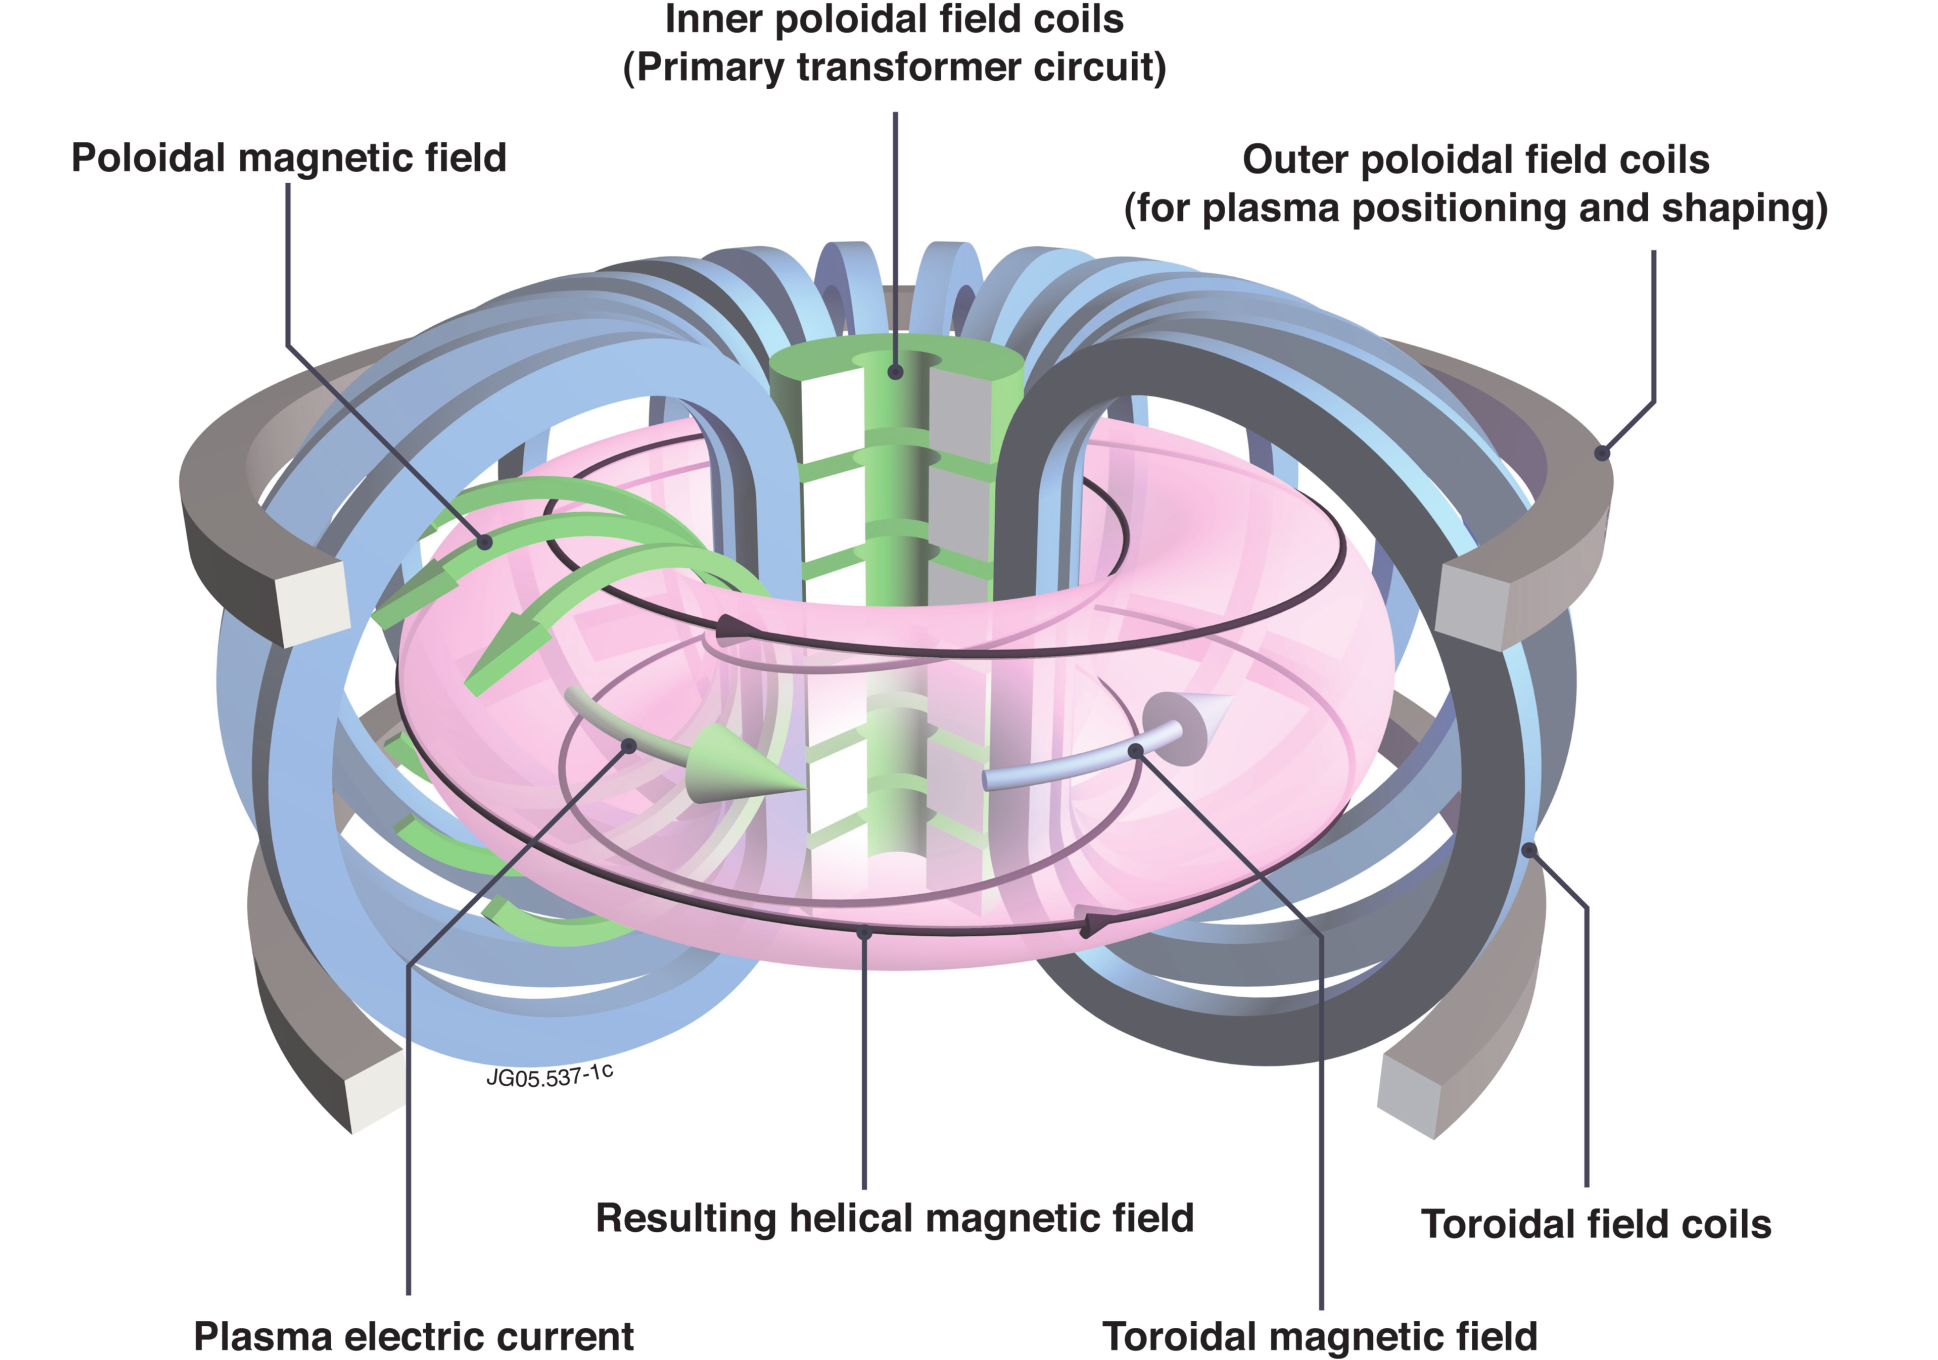
\includegraphics[width=11cm]{figures/tokamak.png}
% 	\caption{Schematic illustration of a tokamak device \cite{eurofusion}.}
% 	\label{Fig:tokamak}
% \end{figure}

% Despite the advanced magnetic geometry of tokamak devices which establish a perfect equilibrium, experimental measurements indicate that large amounts of particles and heat are still transported across the magnetic flux surfaces. This transport is caused by plasma turbulence, which is particularly strong at the boundary of the device. All modern tokamak experiments adopted the \say{divertor configuration}, which is illustrated in \Figref{Fig:sol}. This configuration is achieved by creating a magnetic null point (X-point) in the poloidal plane with a divertor coil carrying a current parallel to the plasma current. Within this point, the magnetic field lines are closed with the last closed flux surface (LCFS), often referred to as the separatrix. The outward region is called the Scrape-Off Layer (SOL), in which the magnetic field lines intersect the divertor plates. Ideally, all plasma leaking from the core through the separatrix into the SOL flows down to the divertor plates where it interacts with the material surfaces, with little to no influence on the fusion process in the core. The poloidal flux expansion near the X-point increases the distance of the magnetic field lines to the divertor plates, letting the plasma cool down before it reaches the material surfaces. Additional precautions, such as tilted target plates, buffers of neutralized gas in front of the target
% (divertor detachment) or installing a second divertor above the plasma column (double-null configuration) are applied in some experiments to reduce the heat flux on the divertor plates further. Despite all these efforts, plasma turbulence leads to highly intermittent bursts of particles and heat propagating through the SOL to the main chamber walls, leading to erosion, damages of sensitive equipment and the release of impurities into the core plasma, where they may degrade confinement and create radiative instabilities. An accurate description for the cross-field transport in the SOL is therefore required in order to predict and handle plasma and heat exhaust in future devices \cite{freidberg2008plasma}.
% \begin{figure}[t]
% 	\centering
% 	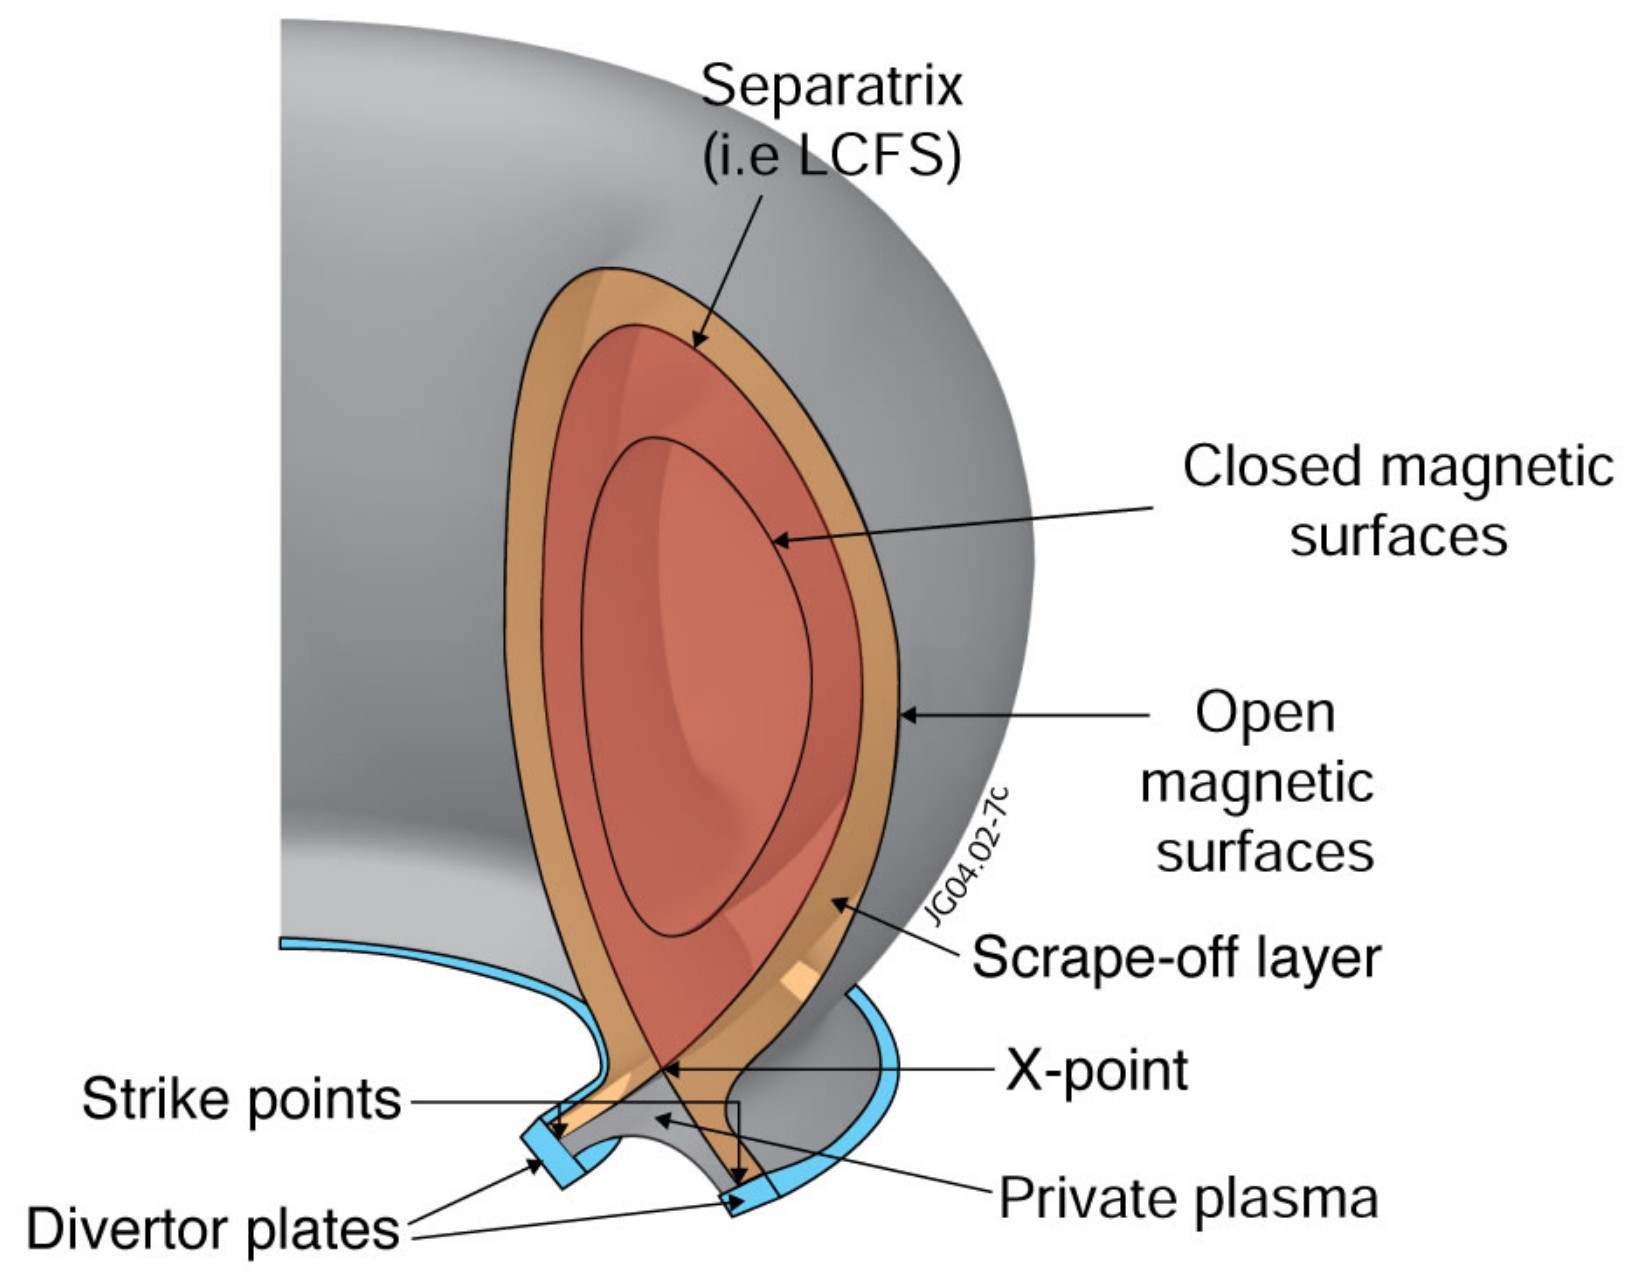
\includegraphics[width=11cm]{figures/sol.png}
% 	\caption{Schematic illustration of the boundary region of a tokamak in a divertor configuration \cite{eurofusion}.}
% 	\label{Fig:sol}
% \end{figure}

% \section{Radial transport in the SOL}
%  Historically, the first attempts to describe cross-field transport in tokamak plasmas used
%  a simple diffusive model in the SOL \cite{connor1999comparison}. In this case the transport follows Fick's law
%  \begin{equation}
%  	\Gamma_\perp = - D_\perp \frac{\partial n}{\partial r},
%  \end{equation}
% where $\Gamma_\perp$ stands for the cross-field particle flux, $D_\perp$ is the diffusion coefficient estimated from the plasma parameters \cite{Bohm1949}, $n$ stands for the plasma density and $r$ for the radial/cross field dimension. This model, however, fails to account for experimental observations, requiring significantly higher diffusion coefficients than expected from classical or Bohm diffusion \cite{lipschultz2002investigation,krasheninnikov2008recent}. Experimental radial profiles in the SOL could only be reproduced by numerical simulations by assuming large cross field drifts or high effective diffusion coefficients $D_\perp^\textrm{eff}$, often referred to as \say{anomalous} diffusion \cite{wesson2011tokamaks}. It was expected that the SOL is dominated by strong flows parallel to the magnetic field, transporting most of the plasma to the divertor targets, resulting in exponential profiles with constant $D_\perp^\textrm{eff}$. These assumptions were refuted by experimental measurements such as presented for the TCV tokamak in \Figref{Fig:garcia_fluc}.
%   \begin{figure}[t]
% 	\centering
% 	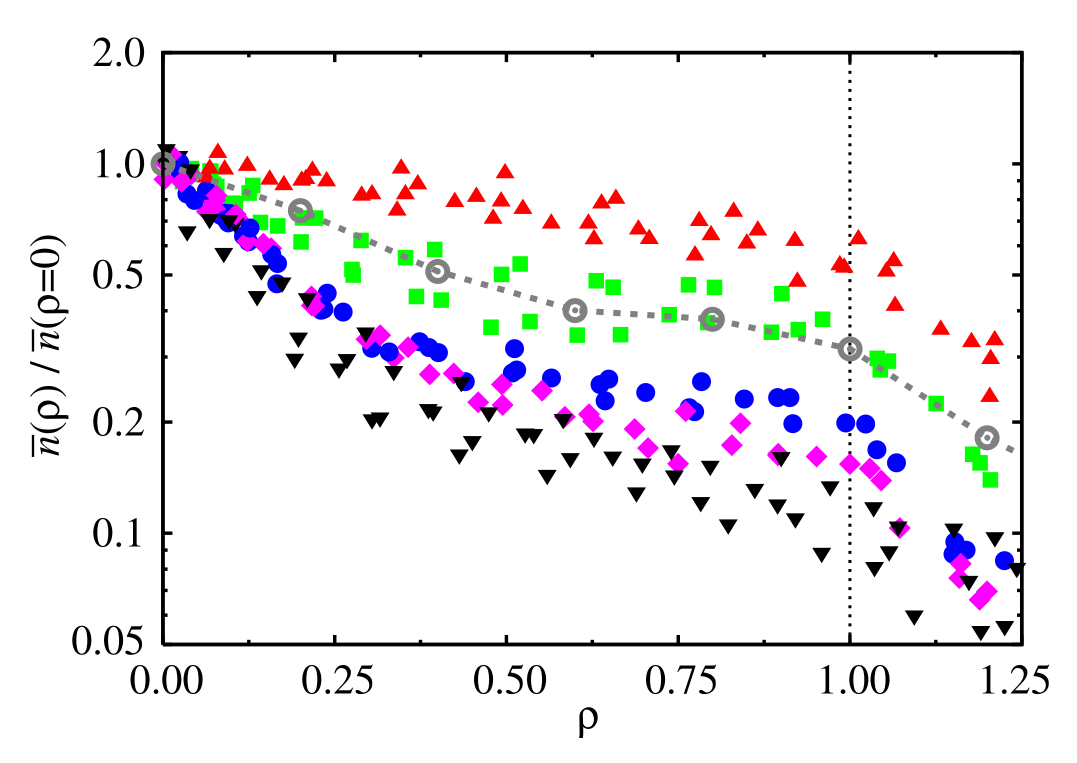
\includegraphics[width=8cm]{figures/garcia_fluc.png}
% 	\caption{Time-averaged, radial profile of the particle density normalized to the separatrix value in the TCV tokamak. The different colored symbols refer to different line-averaged core plasma densities with the black triangles referring to the lowest and the red triangles to the highest value. Reprinted from \cite{garcia2007fluctuations}, with permission from IAEA.}
% 	\label{Fig:garcia_fluc}
% \end{figure}
% Here, the variable $\rho$ stands for the distance to the separatrix and the dashed line indicates the beginning of the wall shadow, the region in which the magnetic field lines interact with the vessel walls. For the lowest line-averaged densities $\overline{n}$ a sharp decay in the density profile is observed close to the separatrix, with a much slower decay radially outwards. These regions are referred to as the near-SOL for the region of steep profiles and far-SOL, respectively \cite{labombard2001particle}. For increasing $\overline{n}$ the break point between these two regions moves radially inwards, resulting in a long decay length in the whole SOL, called broadening \cite{militello2016scrape}. This radial variation is also observed in other tokamak experiments such as Alcator C-Mod, MAST, NSTX, ASDEX, JET and DIII-D \cite{umansky1999modeling,rudakov2005far,militello2013experimental,boedo2014edge,carralero2014experimental,stangeby2000plasma,lipschultz2005comparison}, and in numerical simulations with SOL turbulence codes such as ESEL \cite{naulin2007turbulent}. For a purely diffusive transport this effect requires a significant radial increase of the effective diffusion coefficient as indicated in \Figref{Fig:labombard} for Alcator C-Mod plasmas, questioning the concept of purely diffusive transport.
% \begin{figure}[t]
% 	\centering
% 	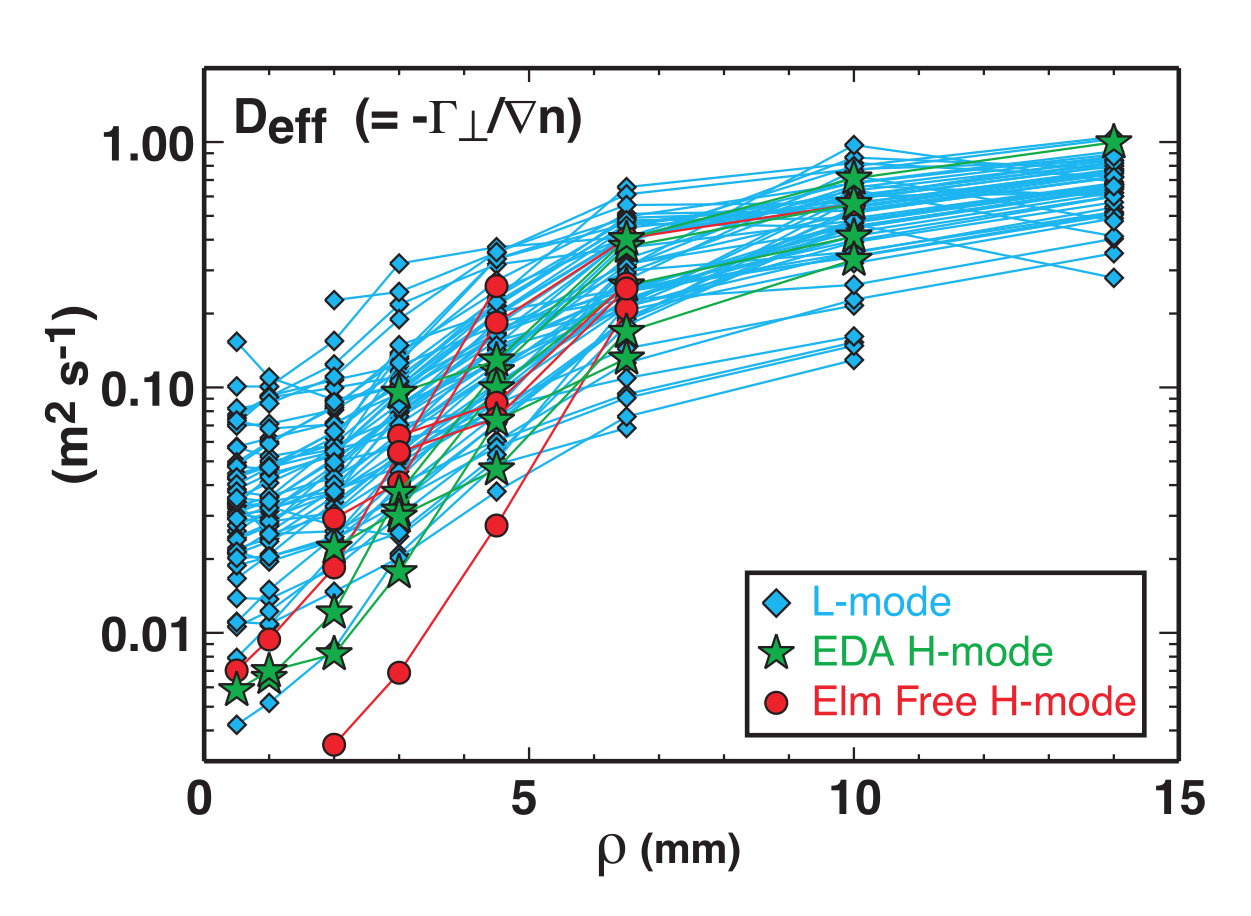
\includegraphics[width=8cm]{figures/effective_diff.png}
% 	\caption{Effective diffusivity profiles for different operational modes of the Alcator C-Mod experiment. The effective diffusion coefficient must vary by several orders of magnitude in order to match purely diffusive transport models. Reprinted from \cite{labombard2000cross}, with the permission of IAEA.}
% 	\label{Fig:labombard}
% \end{figure}
% In the case of the DIII-D experiment, UEDGE transport simulations were unable to find any matching diffusion coefficient \cite{pigarov2002tokamak}. This motivates the introduction of an effective anomalous velocity $v_\perp^\textrm{eff}$ to the diffusion model,
% \begin{equation}
%  	\Gamma_\perp = - D_\perp^\textrm{eff} \frac{\partial n}{\partial r} + v_\perp^\textrm{eff} n.
% \end{equation}
% For an advective-diffusive transport, however, the particle flux would follow a linear relationship with the inverse density scale length $\lambda_n$ \cite{garcia2007turbulent} as
% \begin{equation}
% 	\frac{\Gamma_\perp}{n} =  v_\perp^\textrm{eff} - \frac{D_\perp^\textrm{eff}}{n} \frac{\partial n}{\partial r} = v_\perp^\textrm{eff} + \frac{D_\perp^\textrm{eff}}{\lambda_n}. 
% \end{equation} 
% In experimental measurements, such as for TCV shown in \Figref{Fig:garcia_flux}, no linear relationship can be found. Similar studies on the flux–gradient relation in
% a simple ESEL interchange model of the SOL at
% constant temperatures, shown in \Figref{Fig:naulin},  draw an equivalent conclusion \cite{naulin2007turbulent}.


% These findings clearly indicate that a different model is needed in order to describe turbulence and cross-field transport in the SOL adequately. 
% \begin{figure}
% 	\centering
% 	\begin{minipage}{.48\linewidth}
% 			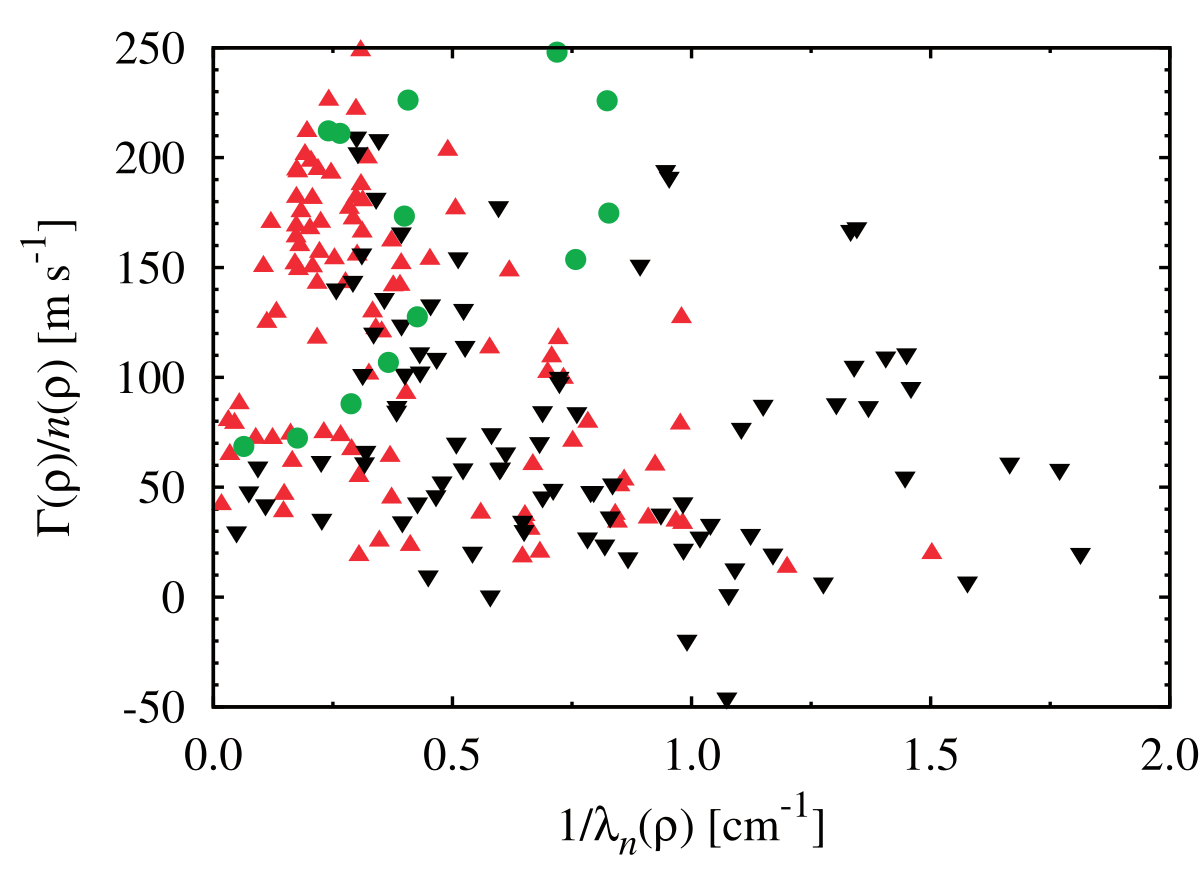
\includegraphics[width=\linewidth]{figures/garcia_flux.png}
% 	\caption{The relationship between the normalized radial particle flux and the inverse density scale length for a range of TCV experiments. Reprinted from \cite{garcia2007turbulent}, with the permission from Elsevier.}
% 		\label{Fig:garcia_flux}
% 	\end{minipage}
% 	\hfill
% 	\begin{minipage}{.48\linewidth}
% 		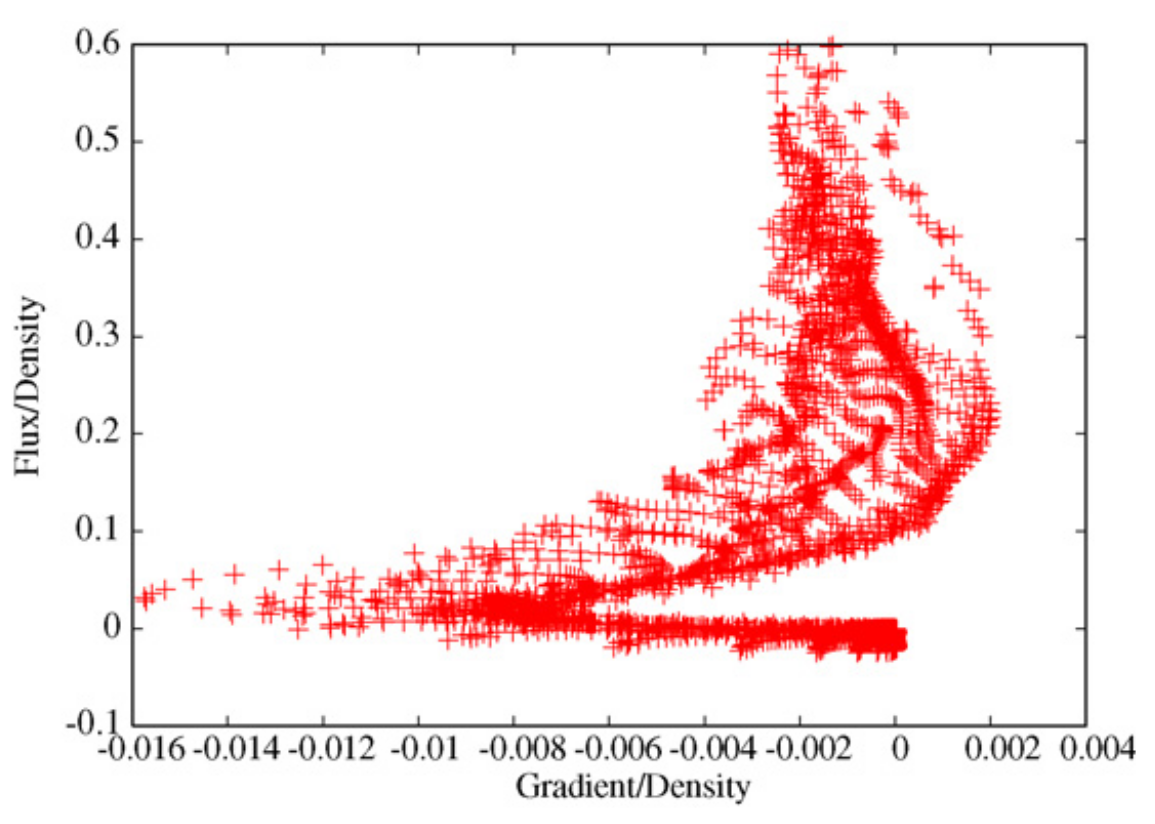
\includegraphics[width=\linewidth]{figures/naulin.png}
% 	\caption{The flux–gradient relation in a simple ESEL interchange model of the SOL at constant temperatures. Reprinted from \cite{naulin2007turbulent}, with the permission from Elsevier.}
% 		\label{Fig:naulin}
% 	\end{minipage}
% \end{figure}


% \section{Intermittent fluctuations in the SOL}
% In the process of finding a better model describing plasma transport in the SOL of tokamak experiments, measurements of the relative fluctuation levels provide additional insight. Among the first experiments investigating this is the Caltech tokamak where fluctuation levels of 10-90\% of the mean were measured in ion saturation current measurements in the edge \cite{zweben1982edge,zweben1983scaling}. Similar observations were made in other experimental devices where these include the TEXT device, shown in \Figref{Fig:wootton}, and in TCV, \Figref{Fig:garcia_rel_fluc}. The fluctuation profiles of the TCV experiment correspond to the time averaged profiles shown in \Figref{Fig:garcia_fluc}. In the low-density case the relative fluctuation levels increase radially in the near SOL and stay approximately constant in the far SOL. Note that the fluctuation levels in the far SOL are independent of the line-averaged core density. For all densities the relative fluctuation levels in the far SOL range between 0.5 and 1, indicating that the broad profiles are dominated by large fluctuations. These findings differ drastically from the plasma core, where fluctuation levels are only around 1\% \cite{mckee2007plasma}. 
% \begin{figure}
% 	\centering
% 	\begin{minipage}{.48\linewidth}
% 		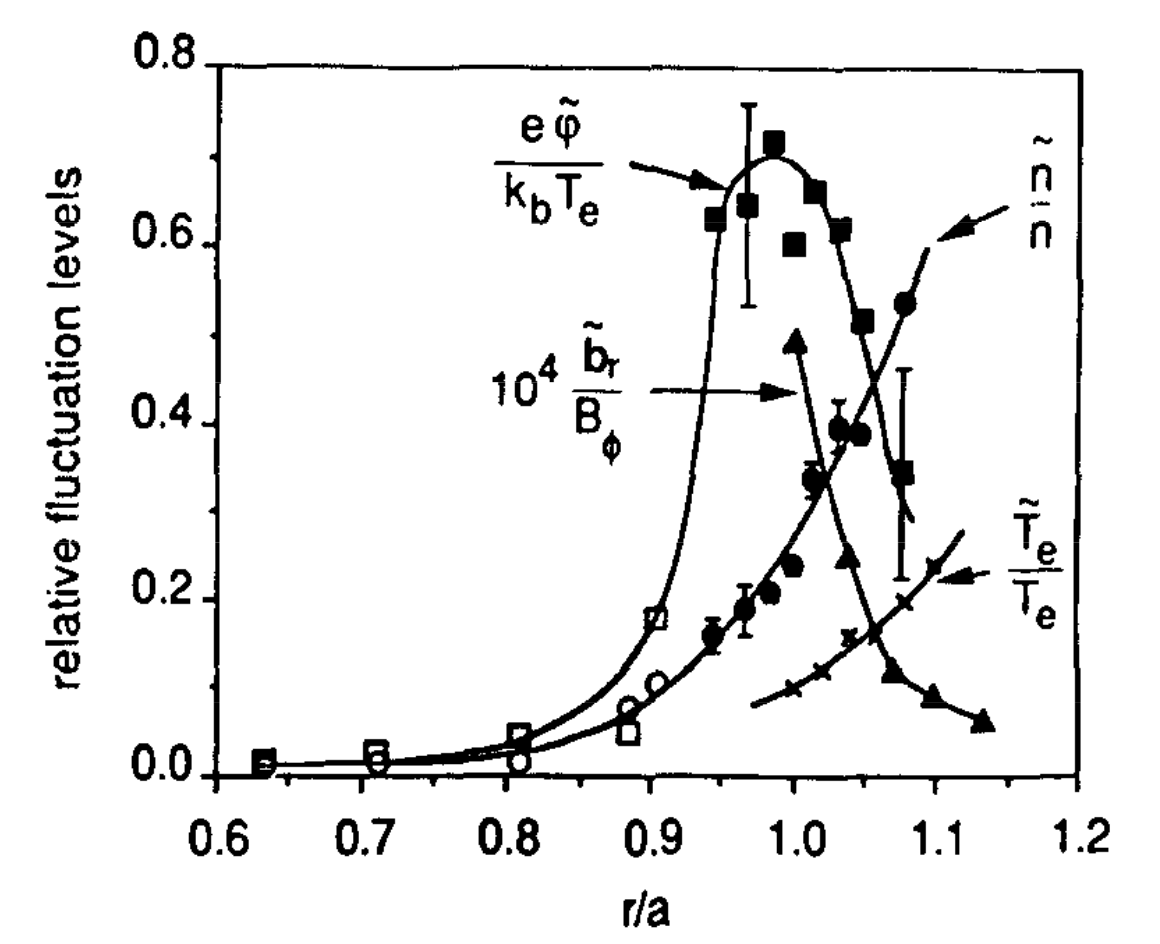
\includegraphics[width=\linewidth]{figures/wootton.png}
% 	\caption{Radial dependencies of fluctuation levels of different plasma parameters in the TEXT tokamak experiment. Reprinted from \cite{wootton1990edge}, with the permission from Elsevier.}
% 	\label{Fig:wootton}
% 	\end{minipage}
% 	\hfill
% 	\begin{minipage}{.48\linewidth}
% 		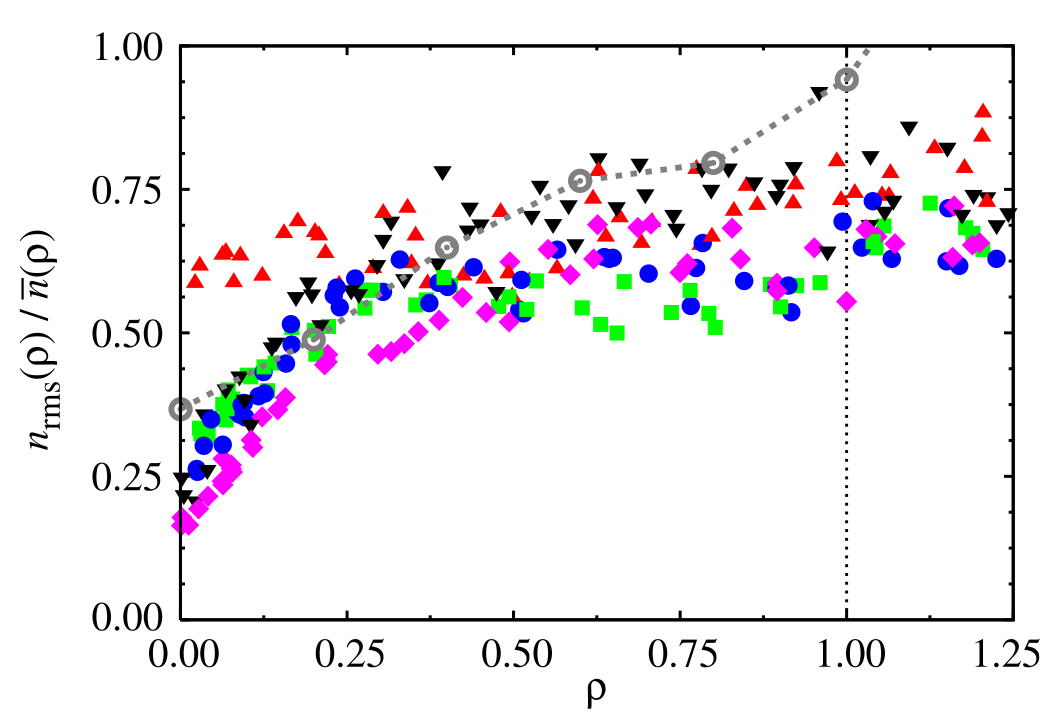
\includegraphics[width=\linewidth]{figures/garcia_rel_fluc.png}
% 	\caption{Radial profile of the relative fluctuation level of the particle density in the TCV SOL. Reprinted from \cite{garcia2007fluctuations}, with permission from IAEA.}
% 	\label{Fig:garcia_rel_fluc}
% 	\end{minipage}
% \end{figure}

% A more detailed picture of SOL fluctuations can be obtained by analyzing time series of the plasma parameters. These time series are typically obtained by Langmuir probes, consisting of a conducting element which is inserted into the plasma and draws a measurable current \cite{langmuir1923positive,mott1926theory}. Another well-known method is Gas puff imaging (GPI), where a puff of neutral gas is injected into the plasma edge, so that excitation radiation can be measured \cite{zweben2017invited}. Examples for time series measured at the outboard mid-plane in the far SOL of TCV, Alcator C-Mod and KSTAR are shown in \Figref{Fig:time_series}. Here, $\widetilde{\Phi}$ stands for the time series $\Phi(t)$ normalized to have zero mean and unit standard deviation. In all three devices, the time series show strongly intermittent positive bursts, which suggests an explanation for the large relative fluctuation levels in the SOL. A stochastic model describing these fluctuations as a superposition of uncorrelated pulses was introduced in 2012 \cite{garcia2012stochastic}. This phenomenological model, known in the context of stochastic processes as the Filtered Poisson Process (FPP), remains to the day of writing this thesis the most accurate statistical description of SOL fluctuations, as all of its major assumptions and predictions agree with the statistical properties of experimental measurements \cite{garcia2013intermittent,garcia2013burst,garcia2015intermittent,kube2016fluctuation,garcia2017sol,kube2018intermittent,garcia2018intermittent,theodorsen2018universality}. A detailed discussion of the FPP model is provided in Chapter 3 of this thesis.
% \begin{figure}[t]
% 	\centering
% 	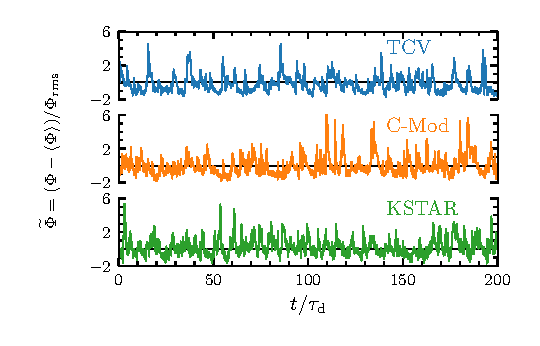
\includegraphics[width=10cm]{figures/compare_ts_alt.eps}
% 	\caption{Fluctuation time series measured from different tokamak experiments. The time is normalized by the characteristic duration time of the underlying bursts. The black line indicates the mean value of the signal. Image courtesy of A. Theodorsen \cite{theodorsen2018statistical}.}
% 	\label{Fig:time_series}
% \end{figure}

% The statistical properties of the fluctuations appear to be remarkably universal across numerous tokamak experiments, confinement modes and plasma parameters. Since positive fluctuations dominate over negative ones, the probability density functions (PDFs) are positively skewed and flattened. \Figref{Fig:antar} shows the PDFs of the ion saturation current measured in the boundary of four different devices, exhibiting almost identical results.  Time series obtained at different radial positions in the boundary region of Alcator C-Mod exhibit close to normal distributions near the separatrix, whereas in the far SOL show increasingly skewed PDFs with an exponential tail towards positive values, as shown in \Figref{Fig:theodorsen_pdf}. Collectively, all of these PDFs are well described by a Gamma distribution with a shape parameter depending on the intermittency of the time series \cite{theodorsen2017relationship}. PDFs with exponential tails towards positive events have also been observed in multiple other devices such as TCV, Tore Supra and KSTAR \cite{antar2001turbulence,antar2003universality,graves2005self,garcia2007fluctuations,garcia2007collisionality,garcia2009blob,garcia2017sol}. The skewness and kurtosis of these time series are exceeding 0 and 3 respectively, as they would be for a normal distribution. A parabolic relationship between skewness and kurtosis has been demonstrated in  \cite{labit2007universal,sattin2009statistics,sattin2009parabolic} which remains consistent with predictions of the FPP model \cite{garcia2016stochastic}.
% \begin{figure}
% 	\centering
% 	\begin{minipage}{.48\linewidth}
% 		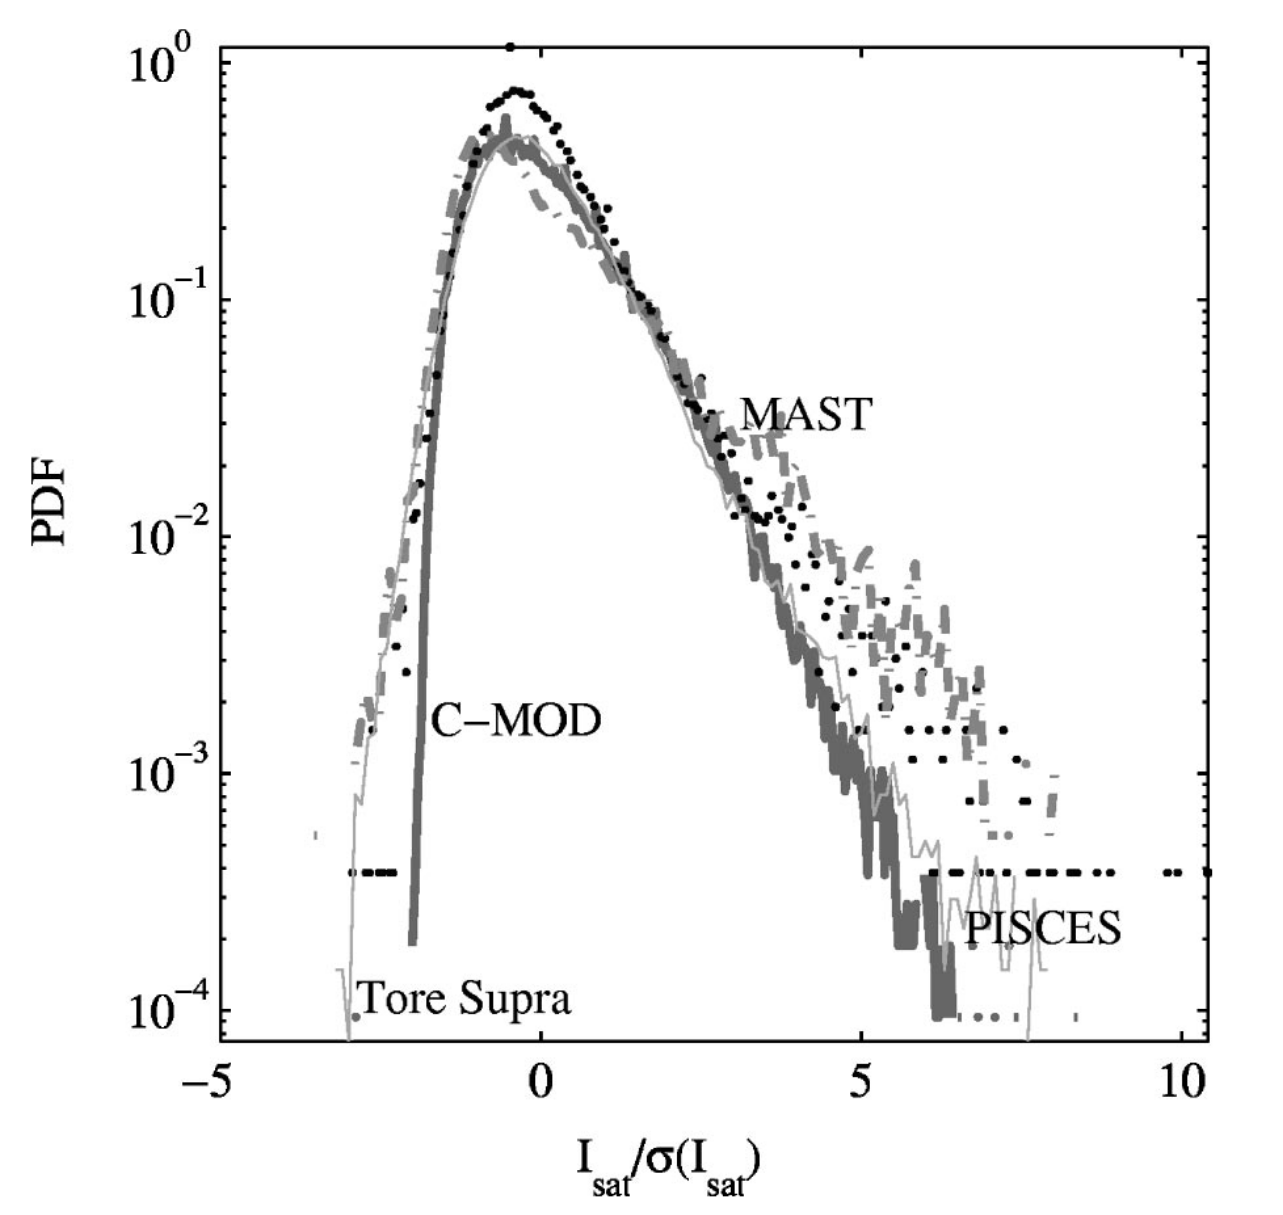
\includegraphics[width=\linewidth]{figures/antar.png}
% 		\caption{PDF of the ion saturation current in the boundary of Tora Supra, Alcator C-Mod, MAST and PISCES. Reprinted from \cite{antar2003universality}, with permission from AIP Publishing.}
% 		\label{Fig:antar}
% 	\end{minipage}
% 	\hfill
% 	\begin{minipage}{.48\linewidth}
% 		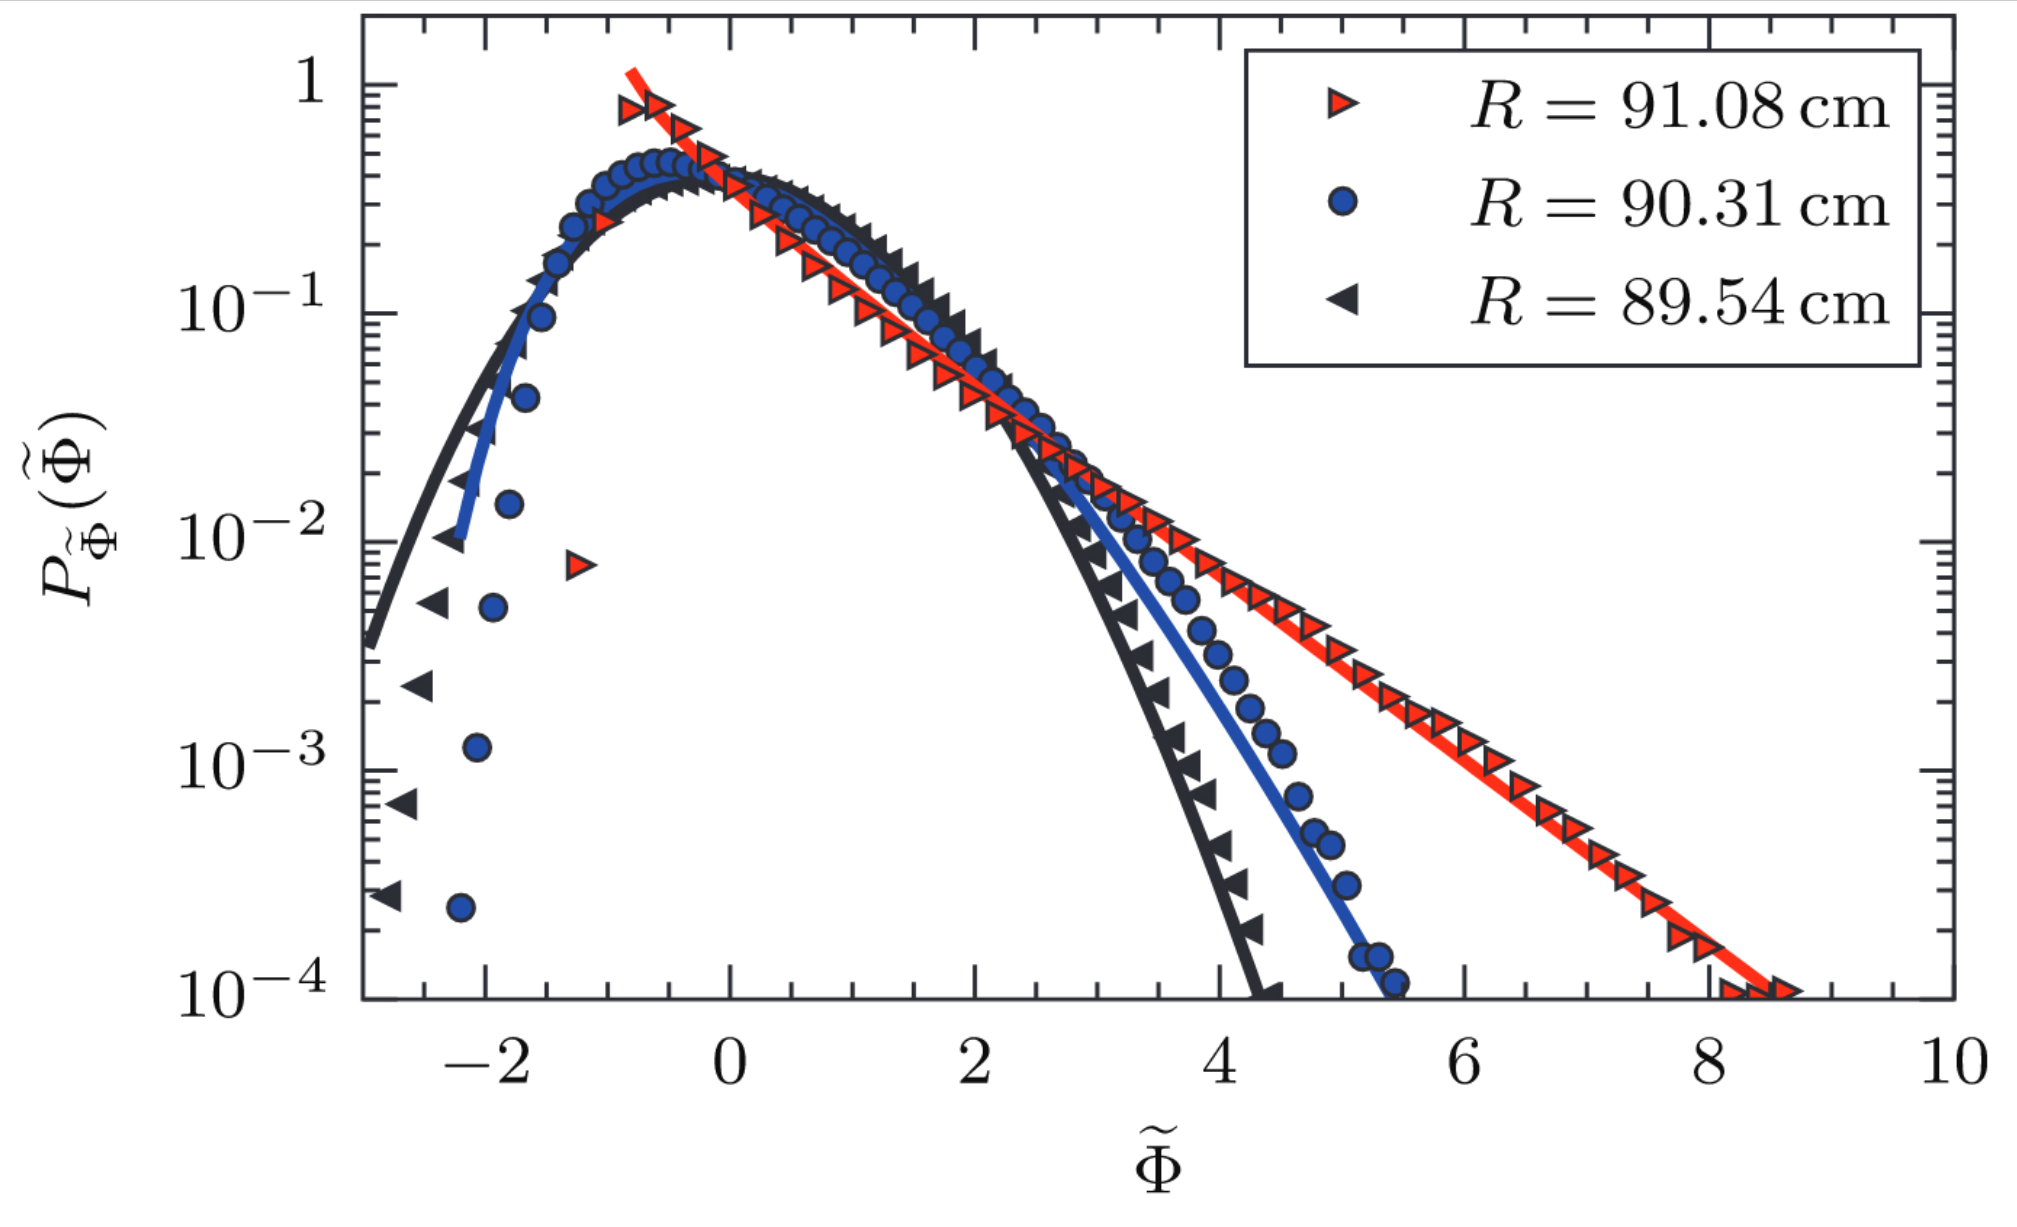
\includegraphics[width=\linewidth]{figures/theodorsen_pdf.png}
% 		\caption{PDFs of gas puff imaging data time series at different radial positions in the boundary of Alcator C-Mod. The full lines represent the predictions of the FPP model. Reprinted from \cite{theodorsen2017relationship}, with permission from IAEA.}
% 		\label{Fig:theodorsen_pdf}
% 	\end{minipage}
% \end{figure}

% The universality of plasma fluctuations in the SOL is also observed in the power spectral densities (PSDs) of the measured time series \cite{pedrosa1999empirical,carreras1999characterization,theodorsen2017relationship,theodorsen2018universality,kube2018intermittent,garcia2018intermittent}. The PSDs of time series for the ion saturation current in a variety of devices are shown in \Figref{Fig:pedrosa}. For a given scaling factor for the frequency axis all PSDs collapse to a single curve. In contrast to the PDFs, the radial position does not seem to have any influence on the PSDs as shown for Alcator C-Mod in \Figref{Fig:theodorsen_psd}. In all experimental measurements the PSD remains flat for low frequencies and shows a power law decay for high frequencies. The analysis of these fluctuations utilizing the FPP framework has shown that the shape of the PSD can be attributed to the shape of the underlying pulses from the time series \cite{garcia2017auto}, providing further support for the stochastic model.
% \begin{figure}
% 	\centering
% 	\begin{minipage}{.48\linewidth}
% 	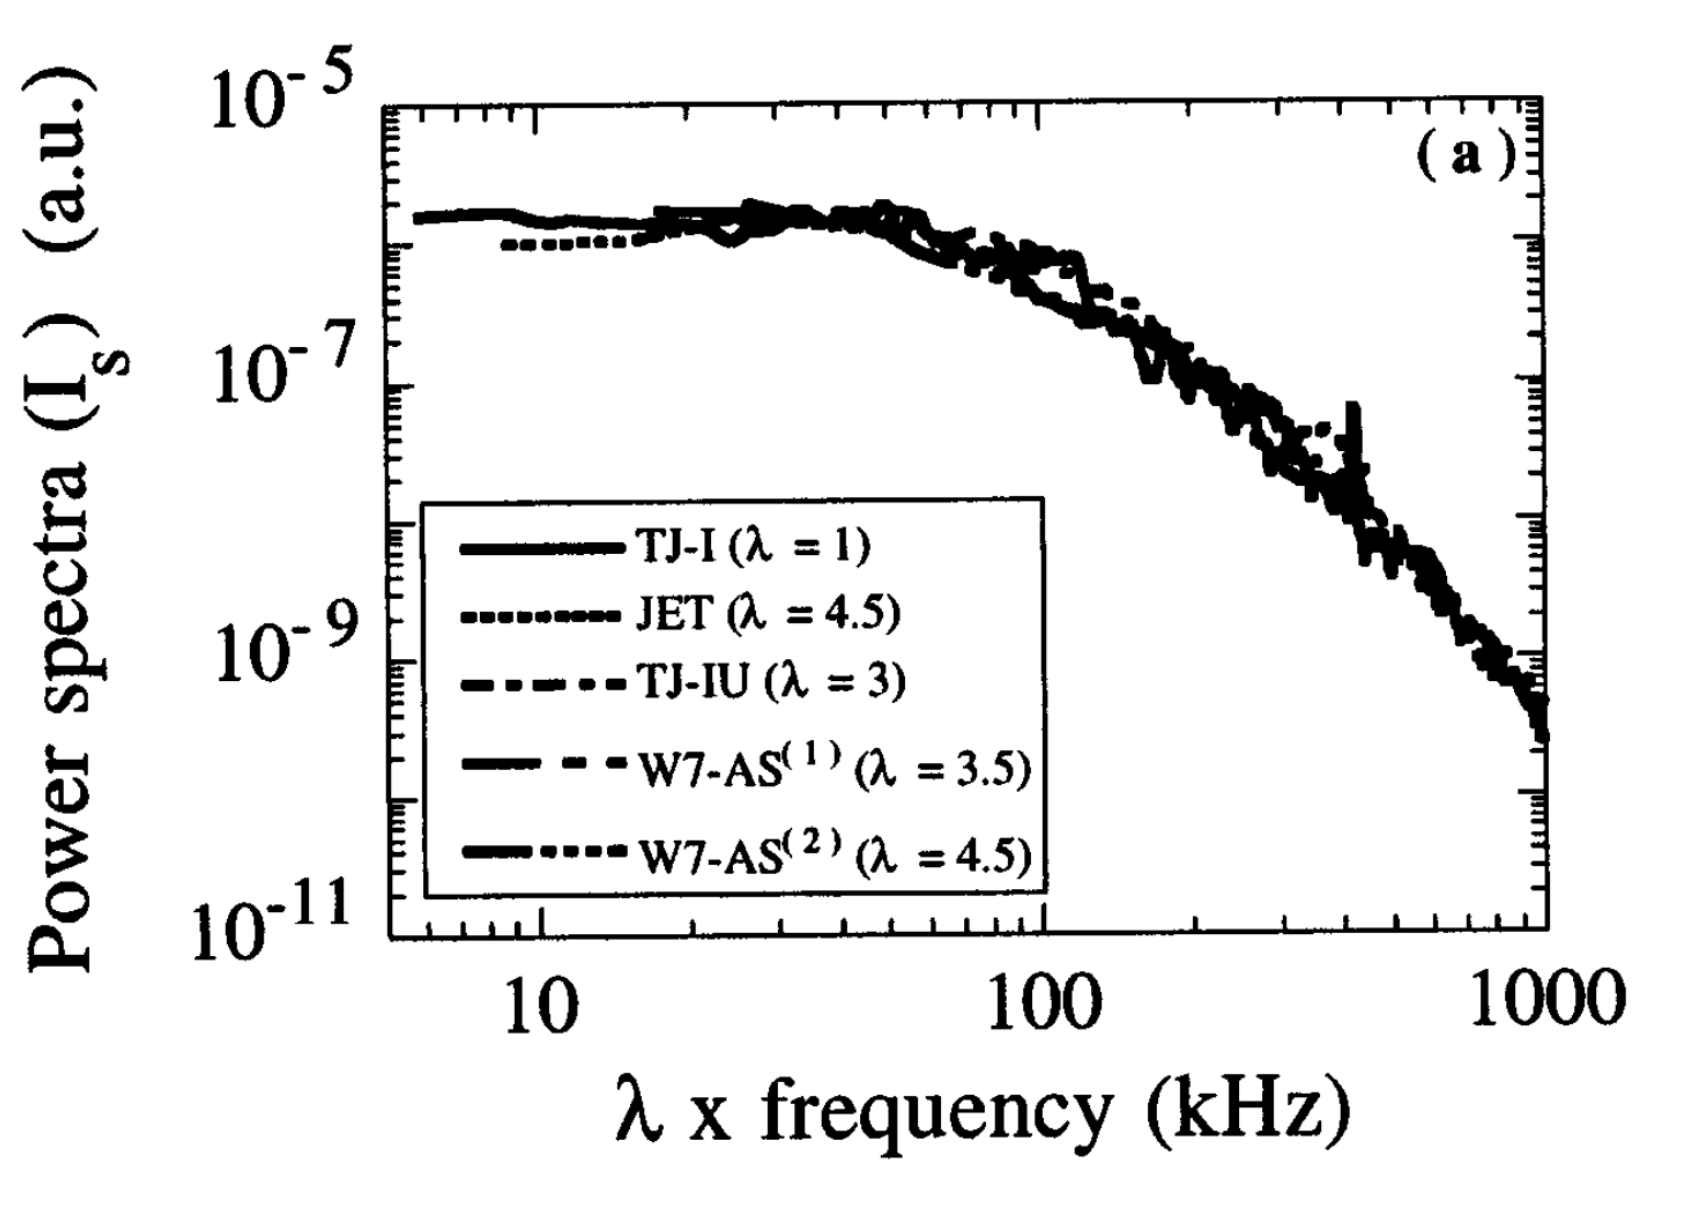
\includegraphics[width=\linewidth]{figures/pedrosa_psd.png}
% 	\caption{PSDs of fluctuation time series of the ion saturation current in various devices. Reprinted figure with permission from \cite{pedrosa1999empirical}. Copyright (1999) by the American Physical Society.}
% 	\label{Fig:pedrosa}
% 	\end{minipage}
% 	\hfill
% 	\begin{minipage}{.48\linewidth}
% 		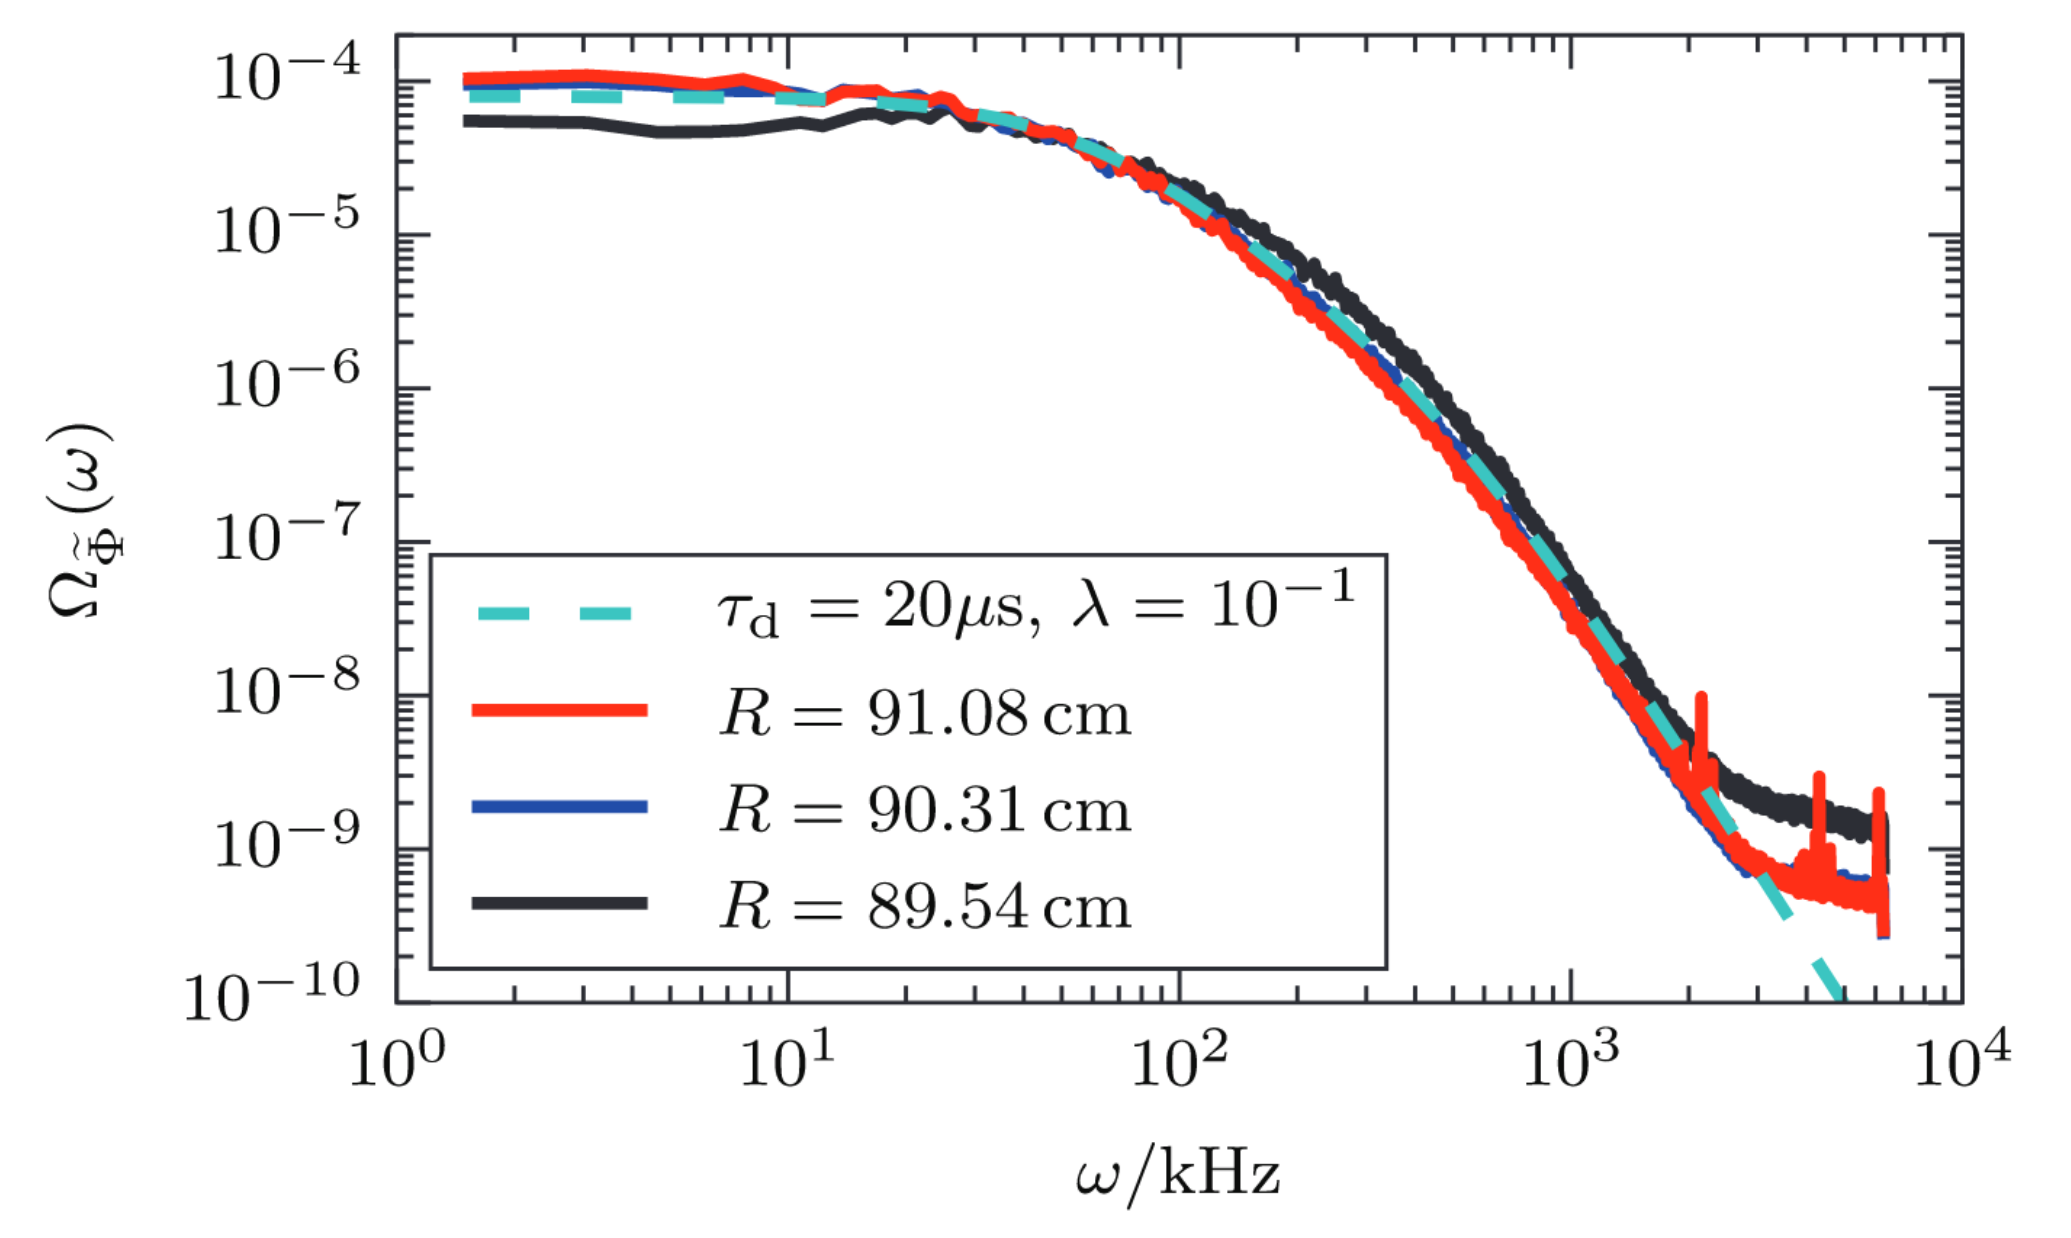
\includegraphics[width=\linewidth]{figures/theodorsen_psd.png}
% 		\caption{PSDs for gas puff imaging time series at different radial positions in the edge of Alcator C-Mod. The broken line shows the FPP predictions. Reprinted from \cite{theodorsen2017relationship}, with permission from IAEA.}
% 		\label{Fig:theodorsen_psd}
% 	\end{minipage}
% \end{figure}

% Apart from stochastic modeling, conditional averaging can be applied in order to reveal the shape of these large-amplitude fluctuations. Hereby all events above a certain threshold, typically 2.5 times the rms-value above the signal mean, are considered and their peak is stored within a time window. The average over all windows is referred to as the conditionally averaged waveform, showing a sharp peak with a short rise and longer decay \cite{antar2003universality,boedo2005edge,garcia2007fluctuations,garcia2007collisionality,garcia2013intermittent,garcia2015intermittent,garcia2017sol,kube2018intermittent,garcia2018intermittent}. The conditionally averaged waveform of time series acquired from the boundary of TCV are shown in \Figref{Fig:garcia2007}. The shape of these large-amplitude fluctuations remain similar for all line-averaged core densities of the experiment and are reproducible by numerical simulations of the two-dimensional ESEL model. \Figref{Fig:theodorsen_CA} shows the agreement of conditionally averaged waveforms for time series measured in different tokamak experiments and compared to an asymmetric, two-sided exponential function. Both the distribution of the maximal amplitude of the conditional structures and the waiting times between two consecutive peaks are found to be exponentially distributed \cite{antar2005scaling,garcia2015intermittent,kube2018intermittent,garcia2017sol,garcia2018intermittent}.
% \begin{figure}
% 	\centering
% 	\begin{minipage}{.48\linewidth}
% 		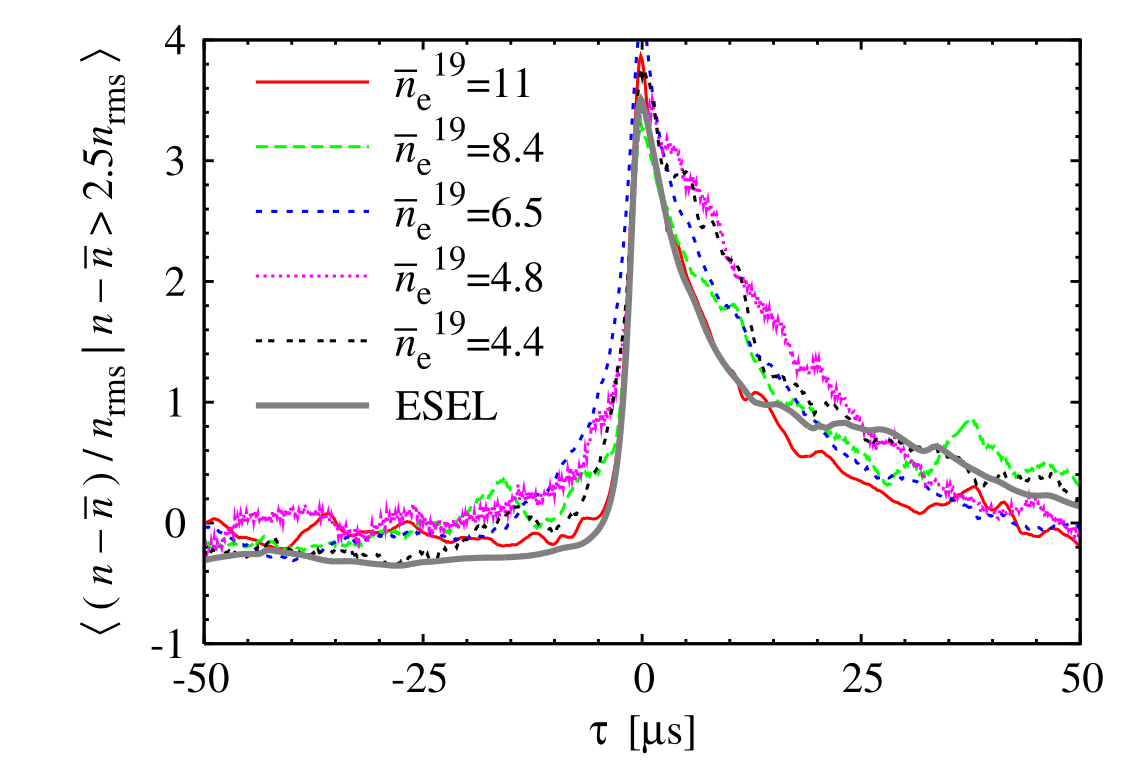
\includegraphics[width=\linewidth]{figures/garcia2007.png}
% 		\caption{Conditionally averaged waveform of particle density time series from TCV and ESEL simulations. Reprinted from \cite{garcia2007fluctuations}, with permission from IAEA.}
% 		\label{Fig:garcia2007}
% 	\end{minipage}
% 	\hfill
% 	\begin{minipage}{.48\linewidth}
% 		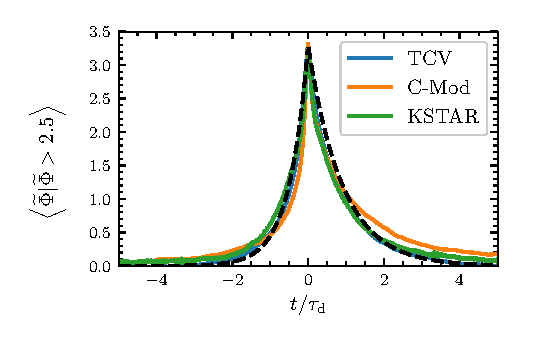
\includegraphics[width=\linewidth]{figures/compare_cav_wf.eps}
% 		\caption{Conditionally averaged waveform for time series measured in the edge of TCV, Alcator C-Mod and KSTAR. The broken line shows a two-sided exponential fit. Image courtesy of A. Theodorsen \cite{theodorsen2018statistical}.}
% 		\label{Fig:theodorsen_CA}
% 	\end{minipage}
% \end{figure}

% In conclusion, the statistical properties of time series measured at the mid-plane boundary of tokamak devices indicate that the SOL is dominated by intermittent structures. In order to investigate the shape of these objects and to gain more information about the physical mechanisms responsible for their transport, stochastic modeling alone, however, does not suffice. 

% \section{Plasma filaments}
% 2D imaging diagnostics such as GPI and wide angle visible imaging reveal that edge transport in the SOL can be attributed to coherent structures. These objects have historically been featured under a variety of names, such as intermittent plasma objects (IPOs), avaloids, solitary vortices and streamers, but are most commonly referred to as filaments or blobs in recent literature. First observations of plasma filaments were made with fast cameras at the Caltech tokamak in the mid 1980's \cite{zweben1985search,zweben1985structure,park1987sj} and with 2D probe arrays in the 1990's \cite{endler1995measurements,endler1999turbulent}. The importance of filaments for edge transport, however, has only been considered at the discovery of the main chamber recycling regime at Alcator C-Mod in 1998 \cite{umansky1998comments}. Since then, plasma filaments have been observed in over 40 devices, including all major tokamak experiments, with a variety of diagnostics \cite{d2011convective}. Filaments typically have a significantly higher density than the surrounding plasma and are aligned to the local magnetic field with their scale lengths much larger in the direction parallel to the magnetic field compared to the perpendicular direction. Filaments have a cross-field size 
% between 2 mm and 10 cm, radial velocity of 0.2 to 2 km/s and a lifetime in the range of tens of $\mu$s \cite{kirk2016mode,dudson2008experiments,zweben2002edge,kube2013blob,myra2006blob,boedo2001transport,silva2004fluctuation,carralero2015experimental,muller2009studies}. Examples of plasma filaments for different confinement modes in the MAST device are shown in \Figref{Fig:ayed}. The elongation of the filaments along the magnetic field, stretching from the upper to the lower divertor is clearly visible.  
% \begin{figure}[t]
% 	\centering
% 	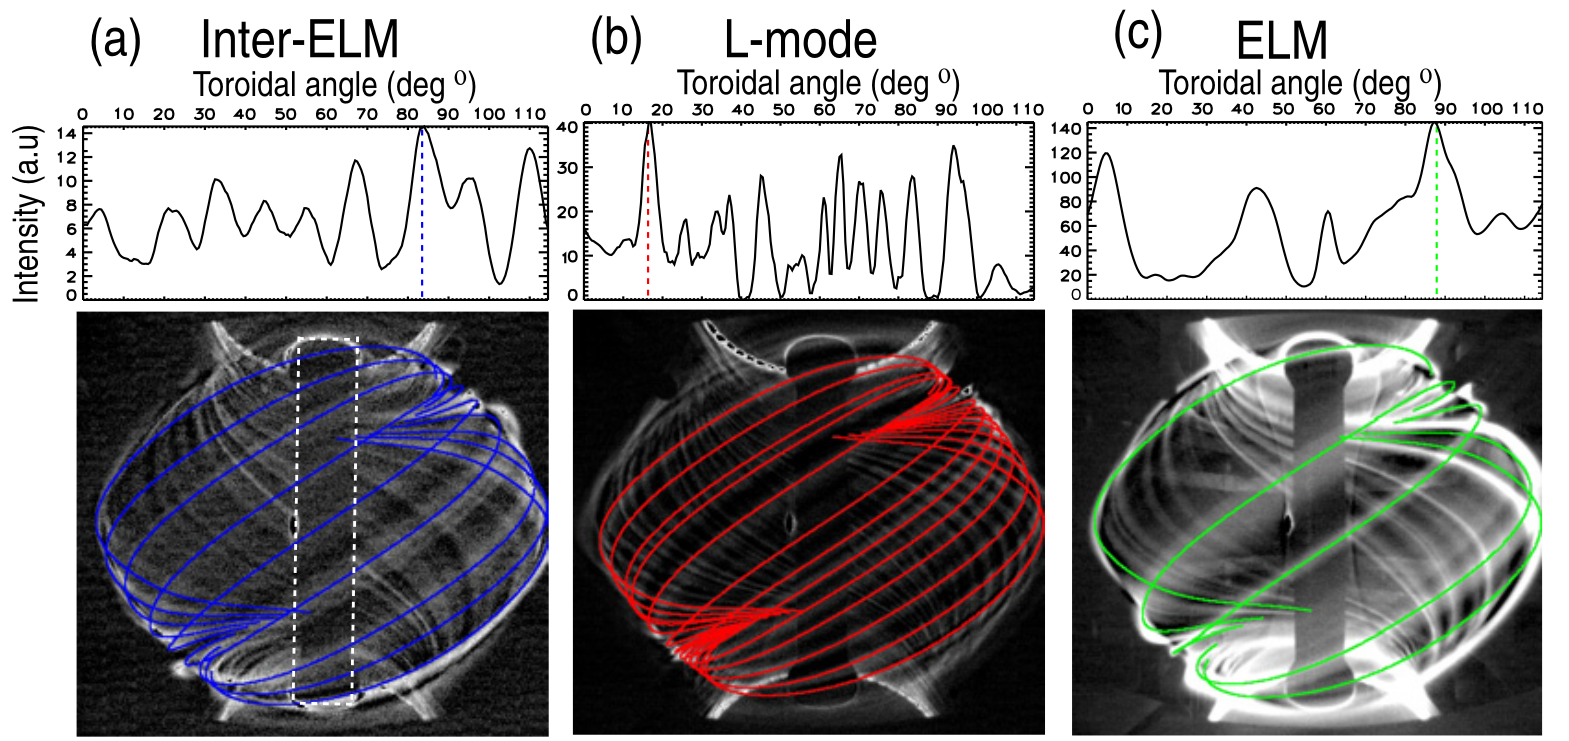
\includegraphics[width=13cm]{figures/ayed_mast.png}
% 	\caption{Wide angle fast visible imaging of inter-ELM, L-mode and ELM
% 		filaments in the MAST device. The panels above show the toroidal variation in emission across
% 		the center column, the peaks are used to label the filaments. Reprinted from \cite{ayed2009inter}, © IOP Publishing.  Reproduced with permission.  All rights reserved.}
% 	\label{Fig:ayed}
% \end{figure}
% Filaments propagate through the SOL due to interchange motion, illustrated in \Figref{Fig:xu}. A simplified model ignoring parallel dynamics explains filament motion as follows: Due to the magnetic geometry at the outboard mid-plane, magnetic gradient and curvature drifts result in a charge polarization, perpendicular to the magnetic field \textbf{B}. This results in an electric field \textbf{E}, transporting the filament in the radial direction with the \textbf{E}$\times$\textbf{B} velocity \textbf{u}$_E$. While the filaments propagate outwards they carry particles and heat much faster than purely diffusive transport would allow, explaining the broad profiles in the SOL.
% \begin{figure}[t]
% 	\centering
% 	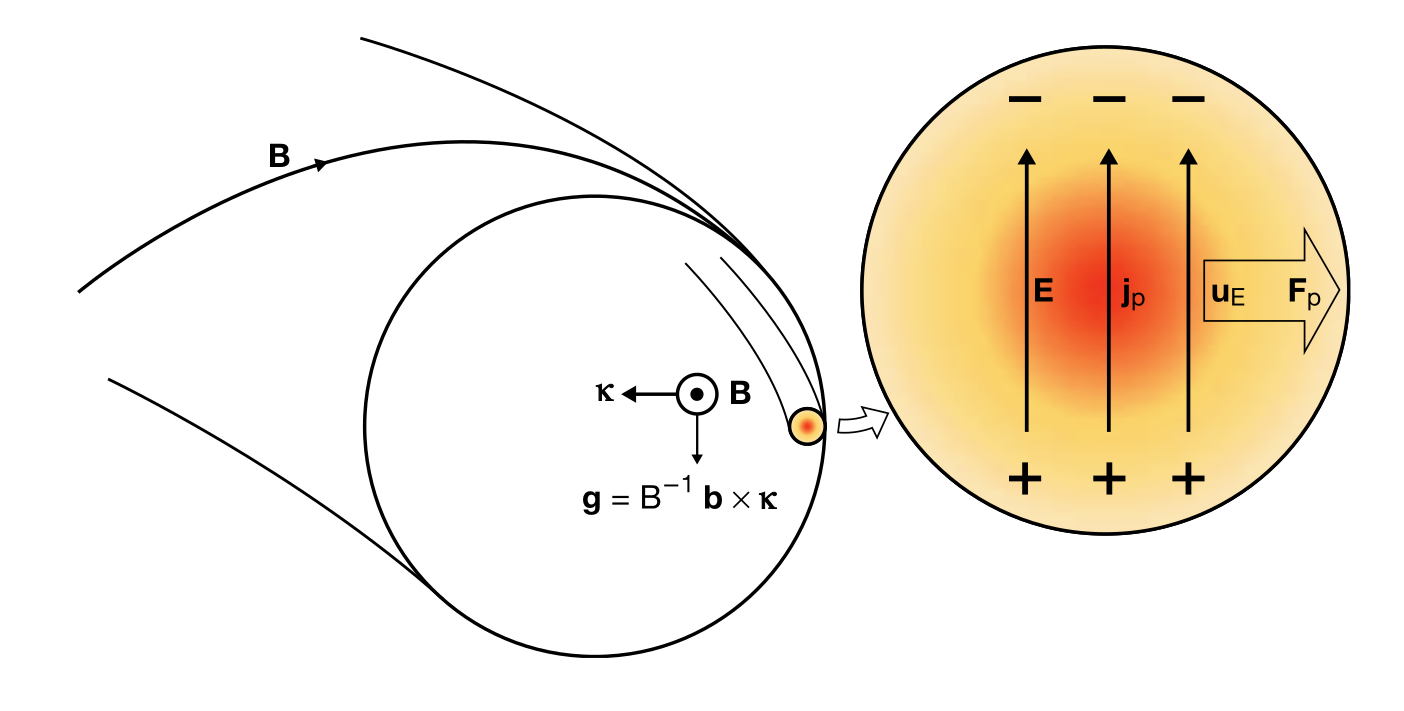
\includegraphics[width=10cm]{figures/xu.png}
% 	\caption{Illustration of charge separation in the filament and the resulting \textbf{E}$\times$\textbf{B} drift, transporting the filament in the radial direction. Reprinted from \cite{xu2010intermittent}, with the permission from AIP Publishing.}
% 	\label{Fig:xu}
% \end{figure}
% \Figref{Fig:maqueda} shows an example of a filament propagating through the SOL of NSTX. Here, the filament is visualized in the plane perpendicular to the field lines. Due to their appearance in the two-dimensional plane, filaments are often referred to as blobs in this context.
% \begin{figure}[t]
% 	\centering
% 	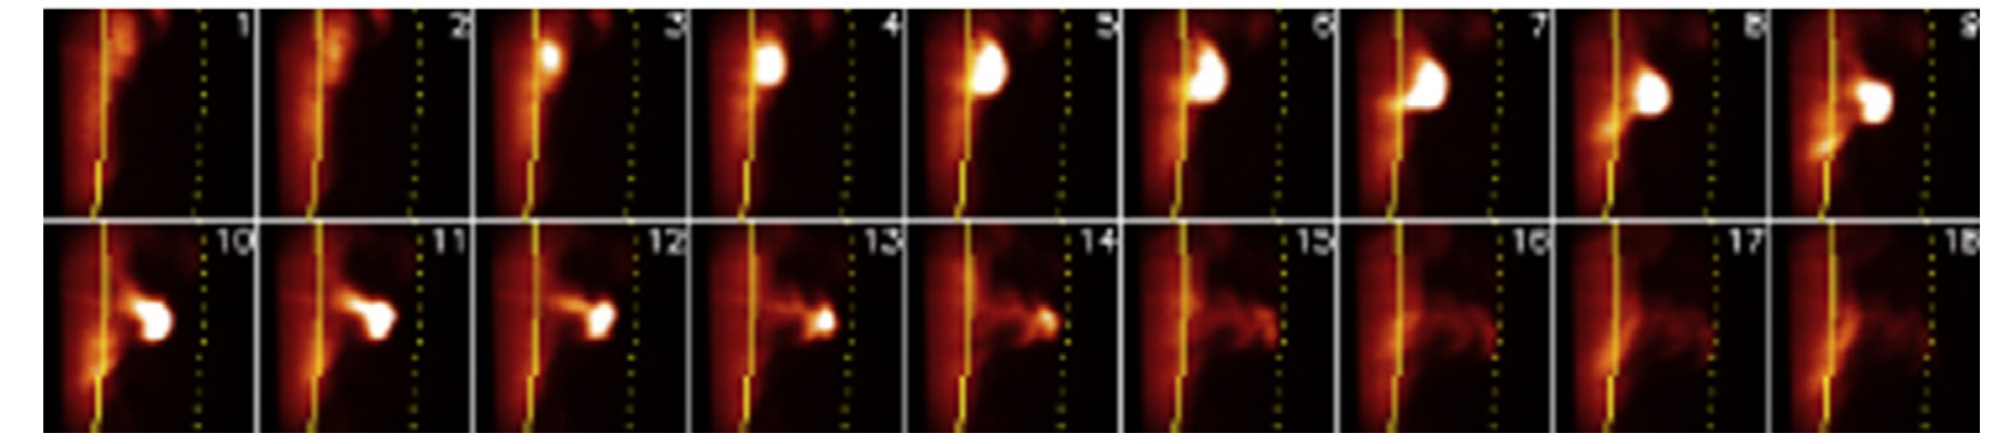
\includegraphics[width=13cm]{figures/maqueda.png}
% 	\caption{Propagation of a blob from the main plasma through the SOL in the NSTX device. Each box shows a $24\times24$ cm portion of the edge at the outer mid-plane and the frame rate is $7 \mu $s. The position of the separatrix is given by the full line and the the wall shadow by the broken line. Reprinted from \cite{maqueda2011intermittency}, with the permission from Elsevier.}
% 	\label{Fig:maqueda}
% \end{figure}

% Measurements using Langmuir probes and GPI simultaneously confirmed that propagating filaments are the same structures that cause intermittent bursts in the time series \cite{grulke2014experimental,zweben2015edge}.  The intermittency of the time series and the length and amplitude of individual bursts are therefore given by the filament parameters. 

% Even though radial blob propagation can be qualitatively understood with the presented two-dimensional model, parallel dynamics must be considered for a more accurate picture \cite{krasheninnikov2008recent}. Since the filament plasma is neutral, the current due to magnetic gradient and curvature drifts must be closed. The charged particles stream along the magnetic field lines until they reach the target plates where the resulting parallel current can close in the plasma Debye sheath. The parallel resistivity of the plasma and the sheath resistivity  limits the magnitude of the parallel current. Alternatively, the current can be closed by polarization currents in the cross-field plane, thereby creating the dipolar electric potential. A schematic illustration of the current paths are shown in \Figref{Fig:krasheninnikov}. The ratio of the current closed through the parallel and perpendicular path determines the strength of the electric field in the filament and therefore its \textbf{E}$\times$\textbf{B} velocity. If the parallel currents are dominant and close mainly in the plasma sheath the filament is said to be in the \say{sheath limited} regime, while in the case where the currents are closed in the cross-field plane, the filament is in the \say{inertial} regime. Analytical velocity scaling laws show that the radial velocity of a filament $v_\perp$ is strongly dependent on its perpendicular size $a$ of a filament \cite{theiler2009cross, angus2012effects}, as
% \begin{equation}
% 	v_\perp(a)  \propto	\begin{cases} 
% 		\sqrt{2 a} \,\, \textrm{for}\,\, a \gg a^*\\
% 		1/a^2 \,\, \textrm{for}\,\, a \ll a^*
% 	\end{cases}	
% \end{equation}
% where $a^*$ is defined as 
% \begin{equation}
% 	a^* = \left(\frac{4 L^2}{\rho_s R}\right)^{1/5}\rho_s.
% \end{equation}
% In this expression $L$ stands for the connection length to the divertor targets, $R$ is the major radius of the tokamak and $\rho_s$ the ratio between the acoustic speed and the ion gyration radius. These velocity scaling laws are reproduced with numerical simulations \cite{garcia2006radial,kube2012effect,kube2016amplitude}. However, it is found difficult to match these laws to experimental observations in both asymptotic limits, as small filaments are difficult to identify and filaments cannot become larger than the SOL width \cite{myra2006blob,kube2013blob}. Relatively good agreement has been found in the toroidal plasma device TORPEX shown in \Figref{Fig:theiler}, showing the joint probability of the filament velocity and cross-field size \cite{theiler2009cross}. Here, the perpendicular width of the filaments is normalized by $a^*$ and the filament velocity by
% \begin{equation}
% 	v^* = \left(\frac{2 L \rho_s^2}{R^3}\right)^{1/5} c_s
% \end{equation} 
% with $c_s$ standing for the ion sound speed.
% The dashed and dotted lines show the ideal scaling laws for the inertial and sheath connected regimes. It is found that the cross-field size of filaments is in between the scale length of the plasma pressure gradient and the particle gyration radius, hence, filaments are often referred to as mesoscale structures.
% \begin{figure}
% 	\centering
% 	\begin{minipage}{.48\linewidth}
% 		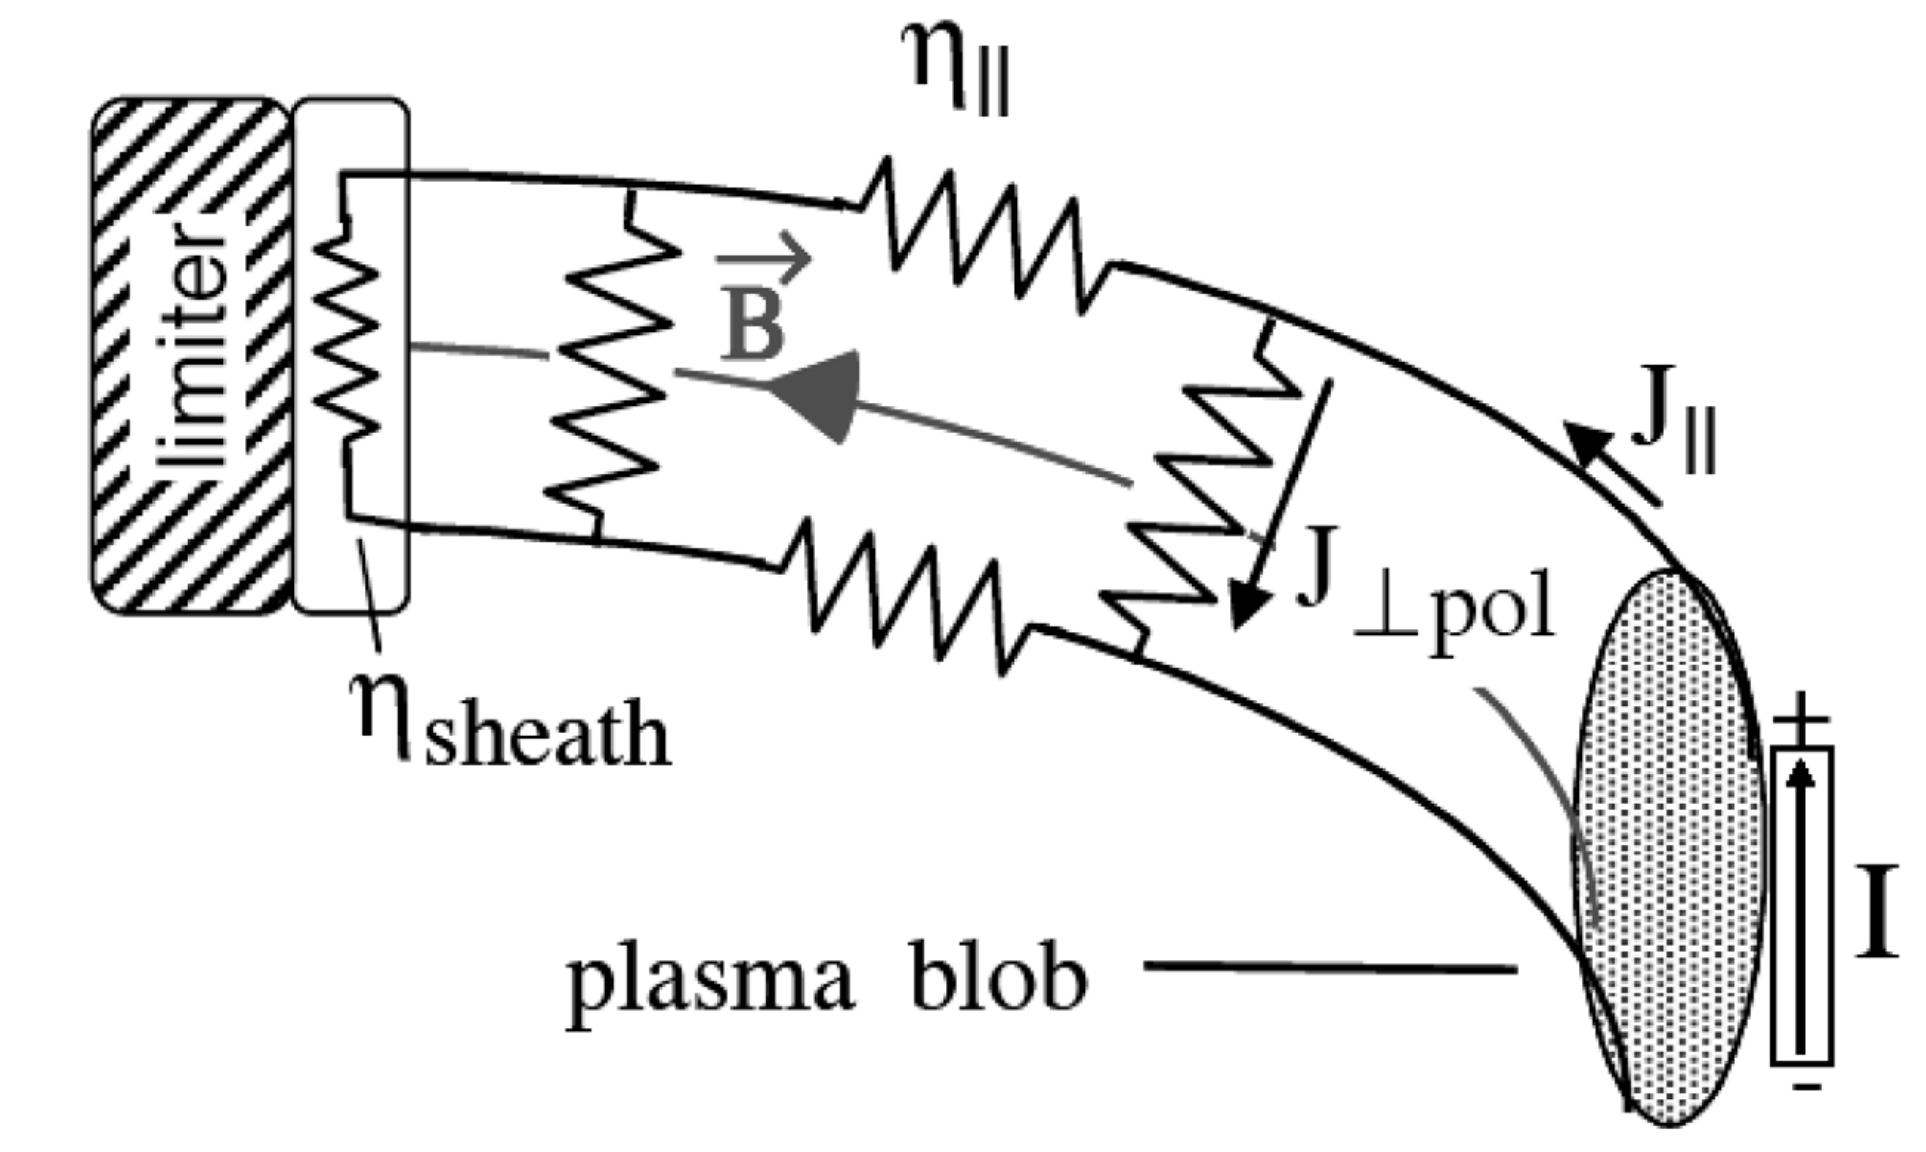
\includegraphics[width=\linewidth]{figures/krasheninnikov.png}
% 		\caption{Schematic illustration of current paths within a filament. Reprinted from \cite{krasheninnikov2008recent}. Copyright © Cambridge University Press 2008.}
% 		\label{Fig:krasheninnikov}
% 	\end{minipage}
% 	\hfill
% 	\begin{minipage}{.48\linewidth}
% 		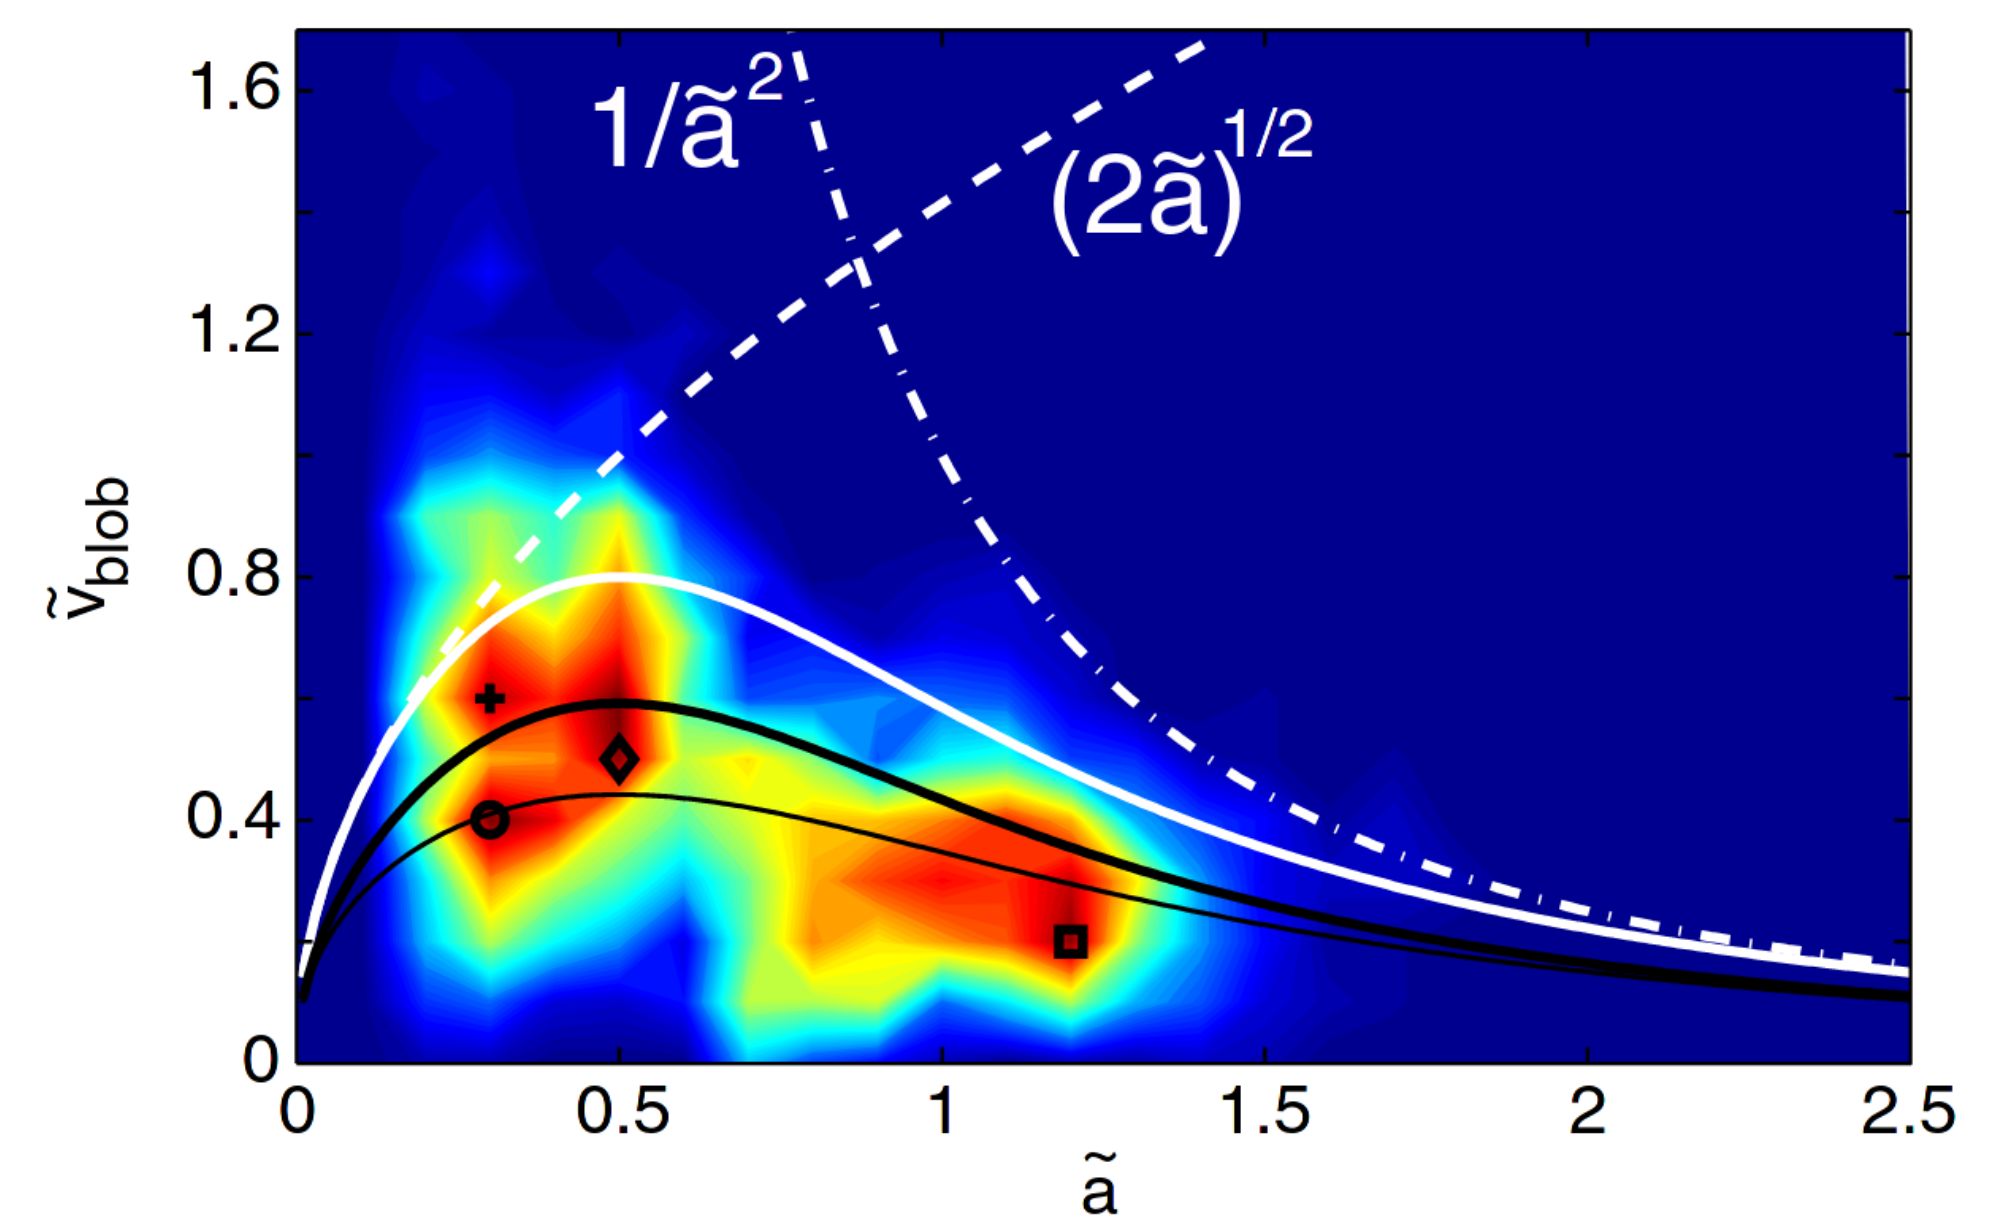
\includegraphics[width=\linewidth]{figures/theiler.png}
% 		\caption{Joint probability of the normalized filament velocity and cross field size in the TORPEX device. Reprinted figure with permission from \cite{theiler2009cross}. Copyright (2009) by the American Physical Society.}
% 		\label{Fig:theiler}
% 	\end{minipage}
% \end{figure}

% Even though filament generation has been extensively studied in tokamak plasmas \cite{terry2005transport,agostini2007study}, simple toroidal plasmas \cite{theiler2008role,muller2007plasma,furno2008experimental,furno2008mechanism} and numerical simulations \cite{garcia2004computations,bisai2005edge,russell2007collisionality,russell2009saturation}, to this day no quantitatively accurate analytical model of filament generation has been developed \cite{d2011convective, krasheninnikov2007generation, krasheninnikov2008dynamics}.  A number of linear instabilities have been identified that are attributed to cause filament generation, namely the interchange, drift-wave, Kelvin-Helmholtz, Rayleigh–Taylor, resistive-ballooning and conducting-wall instabilities \cite{d2011convective,manz2015origin}. Due to the limited understanding of the intricate physics responsible for filament generation in tokamak plasmas, this topic remains a field of active research. 

% \section{Numerical modeling of SOL plasmas}
% As experimental measurements and analytical models for SOL turbulence and plasma filaments face intrinsic limitations, numerical simulations of first principle based models have provided further insight. Due to the complexity of the involved physics, it remains a delicate task to derive models with appropriate approximations that still capture the most relevant physical mechanisms of SOL turbulence. Attempts to model the SOL with gyrokinetic particle-in-cell codes are limited by their enormous computational costs and their dependence on poorly understood boundary conditions \cite{chang2008spontaneous,churchill2017pedestal}. Electromagnetic gyrofluid models have been derived \cite{madsen2013full} and applied for studying temperature dynamics and finite Larmor radius effects on filaments \cite{wiesenberger2014radial,held2016influence}, as well as turbulence in open and closed magnetic field lines \cite{ribeiro2005tokamak,ribeiro2008gyrofluid}. At present, most numerical models for SOL turbulence and filament dynamics originate from the standard plasma fluid transport equations derived by Braginskii \cite{braginskii}. The derivations of the fluid models used in the papers and manuscripts included in this thesis are discussed in Chapter 2. 

% Numerical simulations of SOL plasmas can be categorized into models of saturated turbulence where filament-like structures are created due to nonlinear dynamics, and simulations of explicitly seeded,  isolated filaments. The first self-consistent evolution of a seeded plasma blob in two dimensions has been studied in 2003 \cite{bian2003blobs}, shown in \Figref{Fig:bian}. Here, the blob is initialized as a symmetrical 2D-Gaussian on a constant plasma background. The radial propagation and the evolution of the blob into a mushroom-shaped object with a steep front has been observed.  The radial variation of the density of the blob and its according \textbf{E}$\times$\textbf{B} velocity is shown in \Figref{Fig:garcia_1}. The peak of the radial velocity is trailing the density peak, resulting in a steepening of the blob front. The according temporal evolution is shown in \Figref{Fig:garcia_2}, where the observed pulses have a short rise and long fall time; an observation consistent with the underlying pulses of time series in experiments such as in \Figref{Fig:time_series}. Studies of isolated filaments have been extended to three dimensions, considering dynamics parallel to the magnetic field \cite{angus2012effect,walkden2013characterization,easy2014three,easy2016investigation,militello2016multi,riva2016blob} and have been used to investigate specific physical effects such as electromagnetic effects or finite ion Larmor radius effects \cite{angus2012effect,lee2015electromagnetic,gingell2012transport,gingell2014plasma}. Models for radial blob velocity dependencies on filament amplitudes and sizes have been developed \cite{garcia2005mechanism, garcia2006radial,kube2011velocity,kube2016amplitude}. Simulations of multiple simultaneously seeded filaments discovered that filaments in close proximity interact through the electric potential they generate \cite{militello2017interaction,kendl2018gyrofluid}. A systematical analysis of blob interaction in dependence of the intermittency, defined as the level of blob overlap, is presented in Paper IV.
% \begin{figure}[t]
% 	\centering
% 	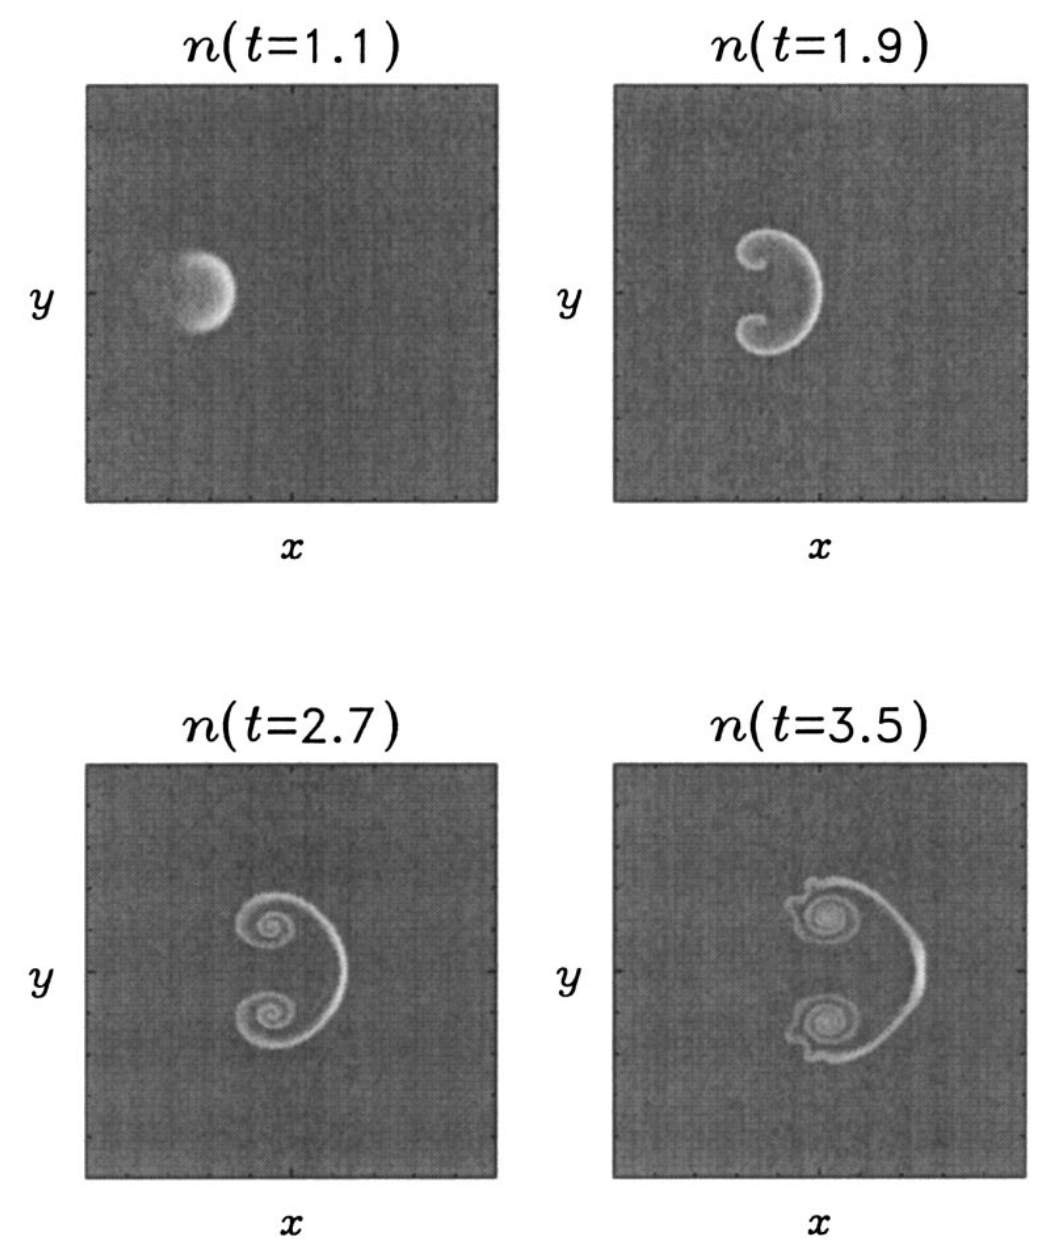
\includegraphics[width=6cm]{figures/bian.png}
% 	\caption{Contour  plot  of  the  evolution  of  a  2D  density  blob. Reprinted from \cite{bian2003blobs}, with the permission from AIP Publishing.}
% 	\label{Fig:bian}
% \end{figure}
% \begin{figure}
% 	\centering
% 	\begin{minipage}{.48\linewidth}
% 		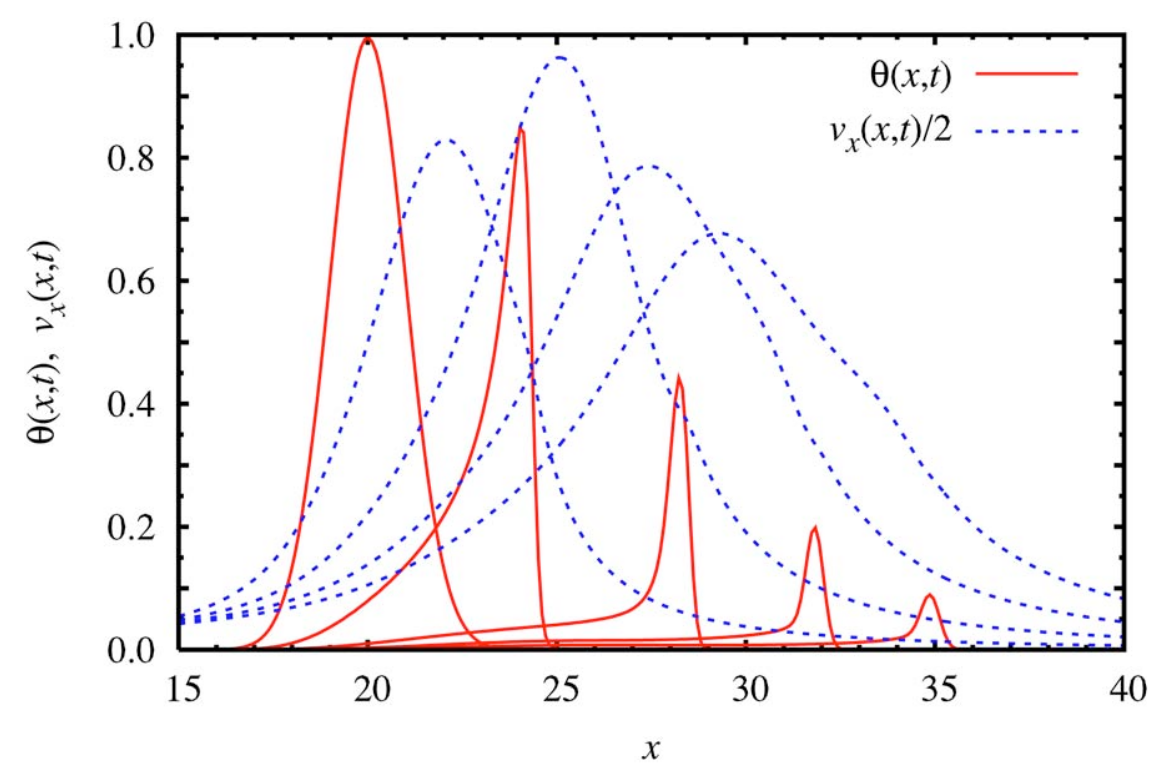
\includegraphics[width=\linewidth]{figures/garcia_blob_1.png}
% 		\caption{Radial variation of the plasma density (full line) and the radial velocity (broken line) at the symmetry axis of a seeded blob. Reprinted from \cite{garcia2005mechanism}, with the permission from AIP Publishing.}
% 		\label{Fig:garcia_1}
% 	\end{minipage}
% 	\hfill
% 	\begin{minipage}{.48\linewidth}
% 		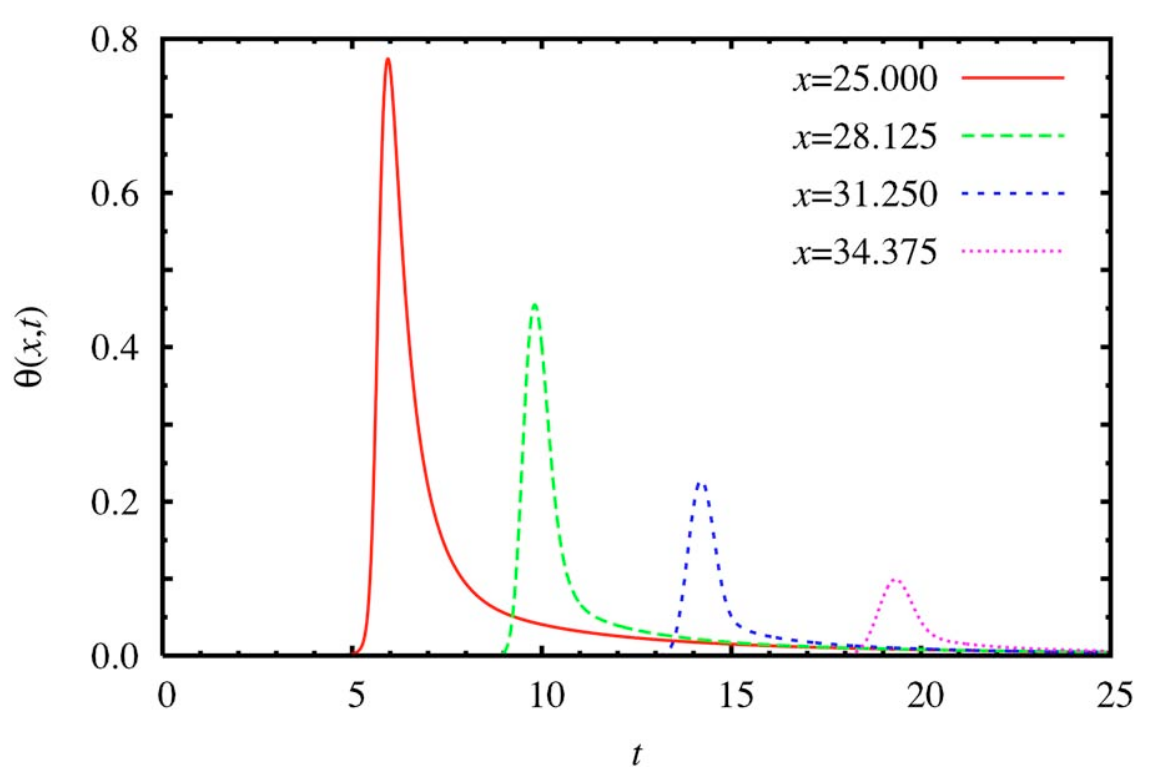
\includegraphics[width=\linewidth]{figures/garcia_blob_2.png}
% 		\caption{Temporal evolution of the plasma density recorded at the symmetry axis at different radial positions. Reprinted from \cite {garcia2005mechanism}, with the permission from AIP Publishing.}
% 		\label{Fig:garcia_2}
% 	\end{minipage}
% \end{figure}

% First attempts of modeling plasma turbulence typically use two-dimensional slab geometries, where curvature effects are modeled by effective gravity terms. Rayleigh–Bénard convection models have been used as a simplified description of the non-linear interchange dynamics in the
% SOL \cite{pogutse1994resistive,beyer1996center,horton1996turbulent,berning2000bifurcations,garcia2003confinement,garcia2003bursting,garcia2006two,decristoforo2020intermittent}. These models have been further extended by including sheath dissipation due to losses along magnetic field lines and drift wave dynamics in the edge region \cite{benkadda1994interchange,sarazin1998intermittent,naulin1999dispersion,garcia2001two,ghendrih2003theoretical,sarazin2003theoretical,garcia2004computations,bisai2004simulation,garcia2005turbulence,bisai2005formation,garcia2006turbulence}. One example for a turbulence simulation in a 2D slab geometry of a model including sheath dissipation is presented in \Figref{Fig:decristoforo}. Plasma streaming from the core into the SOL is modeled as a density source term in the left hand side of the simulation domain. Small perturbations in the plasma density become unstable and result in coherent structures that propagate radially outwards due to the interchange mechanism. The transition from closed to open magnetic field lines is simulated by applying different closures for the parallel dynamics. These 2D turbulence simulations have contributed to the understanding of the stability of filaments in the SOL and were able to reproduce the characteristic PDFs of plasma fluctuations and their radial variations \cite{garcia2005turbulence,militello2012simulations}. Further investigations on the statistical properties in turbulence simulations can be performed by analyzing time series \cite{,naulin2003electromagnetic,naulin2004statistical,garcia2007fluctuations,decristoforo2020intermittent,decristoforo2021numerical} and blob tracking methods in order to investigate filament properties \cite{nespoli2017blob,nespoli20193d,paruta2019blob,decristoforo2020blob}.
% \begin{figure}[t]
% 	\centering
% 	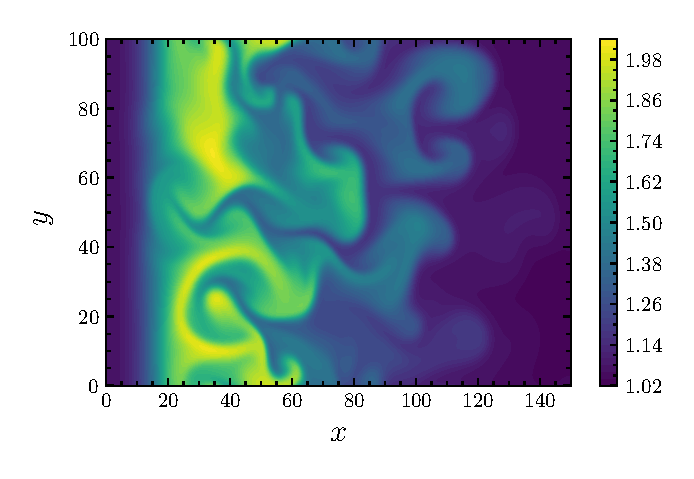
\includegraphics[width=10cm]{figures/decristoforo.eps}
% 	\caption{Snapshot of plasma density of a two-dimensional turbulence simulation. Plasma is injected into the simulations domain at a constant rate and generates blob-like structures due to turbulence. Reprinted from \cite{decristoforo2020blob}, with the permission from AIP Publishing.}
% 	\label{Fig:decristoforo}
% \end{figure}

% Advances in computing power enabled three-dimensional turbulence simulations in the last decade, taking into account the parallel dynamics in SOL plasmas \cite{naulin2005shear,ricci2012simulation,tamain20143d,easy2016investigation,dudson2017hermes,stegmeir2018grillix,Nicholas2021comparing}. Three-dimensional simulations enable implementing realistic geometries and can therefore be used to explore X-point effects and different divertor configurations \cite{nespoli20193d,riva2019three}. Due to their immense computational costs, three-dimensional turbulence simulations have relatively short runs, limiting the amount of statistical analysis that can be performed. 

% A variety of comparisons between the output from numerical simulation codes and experiments have been performed in order to validate simulation codes. These studies mainly focused on the dynamics of individual blob
% structures or on specific physical effects on turbulence and transport. Surprisingly little attention has been attributed to comparisons of fluctuation statistics, considering their universal nature in experiments. The published papers and yet unpublished manuscripts included in this thesis attempt to fill this gap. Here, the main focus lies on utilizing the FPP model, which predicts all major statistical properties of experimental measurements at the outboard mid-plane. By comparing time series from numerical simulations to the predictions of the FPP model one can identify which parameters and assumptions conform to experimental observations. We can thereby gain additional insight and a better understanding of the intricate physics of the boundary of present and future fusion devices.


